\chapter{Reproducibility study}
\label{chap:reproducibility}

The following chapter describes an unpublished collaboration.
My contribution to this project was the scripts to run the HOOMD simulations, and documentation and organization. 
A number of changes and fixes have been initiated by this study, including the following which I am responsible for:
A bug was found in the way Ryckaert-Belleman (RB) dihedrals were converted to OPLS-style dihedrals (mbuild PR 996)
A change in the HOOMD neighborlist API adding the buffer as a required argument prompted a change in the mbuild \lstinline{create_hoomd_forcefield} function. (mbuild PR 988)
Some engines require more precision in the coordinate written to xyz files, so in order to use mbuild's xyz writing capabilities a precision keyword argument was added. (mbuild PR 948)
An correction to Coulomb's constant used in the charge conversion (mBuild PR 1011)
Port the rigid body api to v3 (HOOMD PR 888)
add tail correction for lennard jone pair force (HOOMD PR 1138)

\section{Summary}
 
This is an example of a Chapter. 

\section{Introduction}
%% background
Reproducibility in science is a crucial issue.
If the goal of science is to expand the knowledge of humankind, making sure experiments are reproducible helps to lay a strong foundation for the next discovery.
In computational molecular simulation, where all parameters can be controlled, it would seem an easy task to reproduce an existing work.
Molecular dynamics (MD) and Monte Carlo (MC) simulation are both driven by the core principles of statistical thermodynamics.
Many codes for performing these methods exist each with their own algorithms and implementations, but if each code is correctly using the core principles, the end result should be the same.

This study aims to learn whether different codes can get the same result using the same model.
Within the umbrella of model is the thermodynamic ensemble (e.g., NVT, NPT), the representation of the system (e.g., the force field, constraints, cut offs), and the statepoint (i.e., the pressure, temperature).
In this framework, a "force field" is defined to supply the parameters for a given model.
Other details related to the model: rigid, long-range and charged interactions.

Using the same forcefield may not ensure reproducibility between engines: different engines lack consistency in the functional forms, implementations, and options for handling long-range and charged interactions \citep{Rizzi2020}. 
The energy calculated with a certain code has been found to depend on how the charges are calculated (whether the charge method uses the whole molecule or fragment) and which method is used is often not reported---even differences in Coulomb's constant may cause different results \citep{Shirts2017}.
Due to differences in available implementations in the difference engines there is no one size fits all protocol \citep{Loeffler2018}.
Systematic error was found between engines in as simple a task as calculating the potential energy and density of uncharged molecules in the liquid phase, even between groups using the same engine \citep{Schappals2017}.

This study, a multi-university collaboration, aims to determine what information is necessary to achieve statistically same results across engines.
Researchers from eight universities (see \autoref{tab:unis}) contributed to scripts to initialize and run each of these systems.
Six different engines (see \autoref{tab:engines}) were used to conduct molecular dynamics (MD) and Monte Carlo (MC) simulations.
These scripts will use tools from the Molecular Simulation and Design Framework (MoSDeF) to help with reproducible simulation initialization.
In order to help manage this large data space and submission to various clusters, the Signac framework will be used to programmatically organize the statepoint directories and handle the idiosyncrasies of different cluster schedulers.

\begin{table}
\caption{Universities participating in the study and their abbreviation.}\label{tab:unis}
\centering
\begin{tabular}{ll}
BSU & Boise State University \\
UD & University of Delaware \\
UH & University of Houston \\
UM & University of Michigan \\
UMN & University of Minnesota \\
UND & University of Notre Dame \\
VU & Vanderbilt University* \\
WSU & Wayne State University
\end{tabular}
\end{table}

\begin{table}
\caption{Simulation engines used in the study along with the publications in which the engine is described, simulation type, and the research group resonsible for that engine.}\label{tab:engines}
\centering
\begin{tabular}{llll}
Code      & Type & Ref             & Group   \\ \hline
Cassandra & MC   & \cite{Shah2017} & UND     \\
GOMC      & MC   & \cite{Shah2017} & WSU     \\
Gromacs   & MD   & \cite{ABRAHAM201519, Pall2015, 10.1093/bioinformatics/btt055, Lindahl2001, BERENDSEN199543, https://doi.org/10.1002/jcc.20291, Hess2008} & VU      \\
HOOMD     & MD   & \cite{Anderson2020, Nguyen2011a, Glaser2020a, Lebard2012} & BSU, UM \\
LAMMPS    & MD   & \cite{LAMMPS} & UD, VU  \\
MCCCS     & MC   & \cite{C8SC05340E,Josephson2019} & UMN    
\end{tabular}
\end{table}

This study is still ongoing, so some of the data shown in this chapter may be unfinished or incomplete. 
I will focus most on the simulations run using HOOMD, as this is the part of the study I am responsible for.
I will also try to distill what we have learned, through the numerous hurdles we have discovered and overcome. 
This project involved a great deal of collaboration and discussion.
Although the systems studied are very simple, we ran into many challenges:
Keeping consistent units, sharing data, and many unexpected hurdles to get consistency between engines due to the different available functions in each engine. % wording?
Choosing what information to store and how to format that information so it is readable by one analysis script. 
The benefit of this study is that it provides comprehensive information: the results obtained and the exact code ran to obtain them. 
These data can be used by other simulators to validate their work.
These workflows can also serve as valuable examples. 
At the time this study started, HOOMD v3 was still in beta, so the HOOMD part of this project can serve as a valuable example of how to (1) run atomistic simulations consistently with other engines, (2) initialize rigid bodies and bond constraints using the MoSDeF framework (this workflow is currently the only available example of how to initialize rigid bodies on an existing system), and (4) log individual energies such that they can be compared to other engines. 
We have learned that even when you control every step of the initialization process, there are still so many additional user-tuned parameters in each engine that guaranteeing reproducibility requires careful thought.

\section{Models}
The systems which are studied are small, simple, and chosen to demonstrate simulation in systems with varied degrees of complexity:
\begin{figure}[h!]
    \centering
    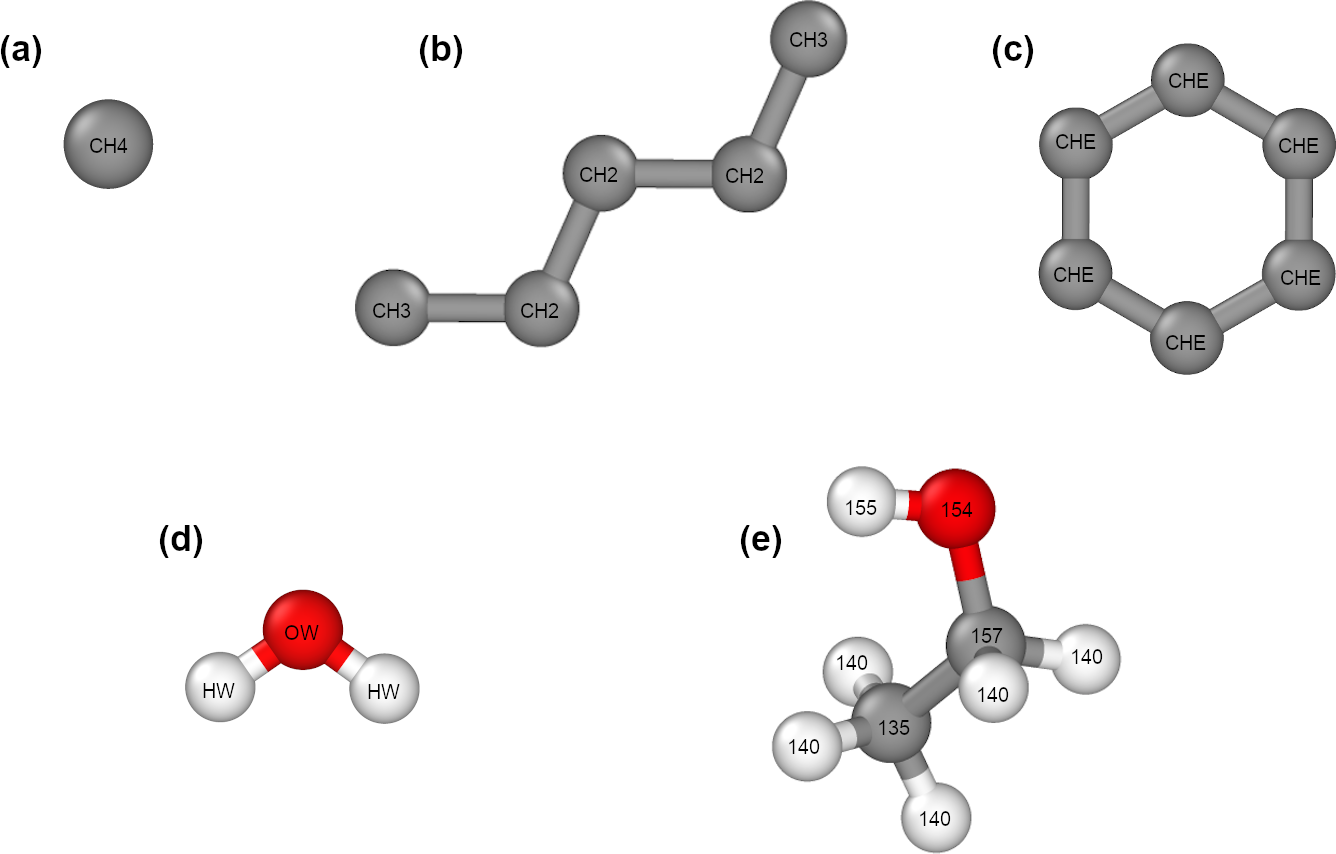
\includegraphics[width=\linewidth]{figures/rep_study/models.png}
    \caption{Structures of the five models with the atoms types labelled: (a) TraPPE-UA methane, (b) TraPPE-UA pentane, (c) TraPPE-UA benzene, (d) SPC/E water, (e) OPLSAA ethanol}\label{fig:models}
\end{figure}
The TraPPE united-atom (UA) forcefield was applied to UA methane (see \autoref{fig:models}a) and pentane (see \autoref{fig:models}b) models to investigate the simplest case of only Lennard-Jones interactions and a linear molecule with bonds, angles and dihedrals \citep{Martin1998}.
TraPPE-UA was also applied to a UA benzene model (see \autoref{fig:models}c) to investigate rigid ring structures.
(We initially tried a flexible model based on TraPPE-UA, but some engines were not able to get this model to run \citep{Yiannourakou2019}.)
The SPC/E water model (see \autoref{fig:models}d) was used to investigate a rigid molecule with electrostatics \citep{Berendsen1987a}.
Finally, the most complex system, the OPLS all-atom (AA) forcefield was applied to ethanol (see \autoref{fig:models}e) to investigate a fully atomistic, charged molecule \citep{Jorgensen1988}.
The step-wise, increasing complexity in these systems was later very useful for pinpointing the source of a discrepancy between engines.

The nonbonded interactions were modelled as Lennard-Jones (LJ) interactions. 
And charged interactions are computed via the particle particle particle mesh (PPPM) method as described in \citet{Darden1993} and \citet{Lebard2012}. 
The bonded interactions were modelled as harmonic bonds, harmonic angles, and OPLS style dihedrals.
The forcefield parameters for TraPPE-UA and OPLS-AA are provided with Foyer \citep{foyer}. 
The non-bonded potential parameters for SPC/E water can be found in \autoref{tab:water}. 
The non-bonded TraPPE-UA potential parameters used for benzene can be found in \autoref{tab:bz_nonbond}. No bonded potentials were used for either water or benzene as both molecules were modelled as a rigid bodies \citep{Nguyen2011a, Glaser2020a}. 

As is common in molecular simulation, the Lennard-Jones equation (Equation~\eqref{lj}) was used to model the non-bonded potentials between particles.
To save computational resources, it is common to truncate the potential at a certain distance, and, as a discontinuity in the potential energy can issues in energy conservation, there exist various smoothing schemes for handling values beyond the cutoff.
\begin{alignat}{3}
U_{LJ}(r) & = 4\epsilon\bigg[\bigg(\frac{\sigma}{r}\bigg)^{12} - \bigg(\frac{\sigma}{r}\bigg)^{6}\bigg]; && r<r_{cut} 
    \label{lj} \\
& = 0; && r>=r_{cut}
    \nonumber
\end{alignat}
Let us define three cases for how the potential beyond the cutoff is handled: hard, shifted, and long-range correction (LRC). 
In the "hard" cutoff scheme, the potential is simply set to zero beyond $r_{cut}$ with no smoothing regardless of the potential’s value at $r_{cut}$.
The "shifted" cutoff scheme shifts the entire potential by the potential value at $r_{cut}$ (a constant) such that the potential at $r_{cut}$ is zero.
Finally, the "LRC" scheme applies a correction to the total energy and pressure based on the particle number densities beyond $r_{cut}$.
At the time this study was initiated, the only options for handling the cutoff shared between all engines were the "shifted" and "hard" schemes.
As discussed in \autoref{sec:cutoff} it was found that these cutoff schemes were not adequate for equilibrating to the correct density or agreement between MD and MC.
So in order to use the "LRC" scheme in HOOMD I contributed the tail correction calculations for the LJ pair object. 
The tail correction code was included in the HOOMD v3.0.0 release.
All simulations in the main project use the "LRC" cutoff scheme.

\section{Methods}

\begin{figure}[h!]
    \centering
    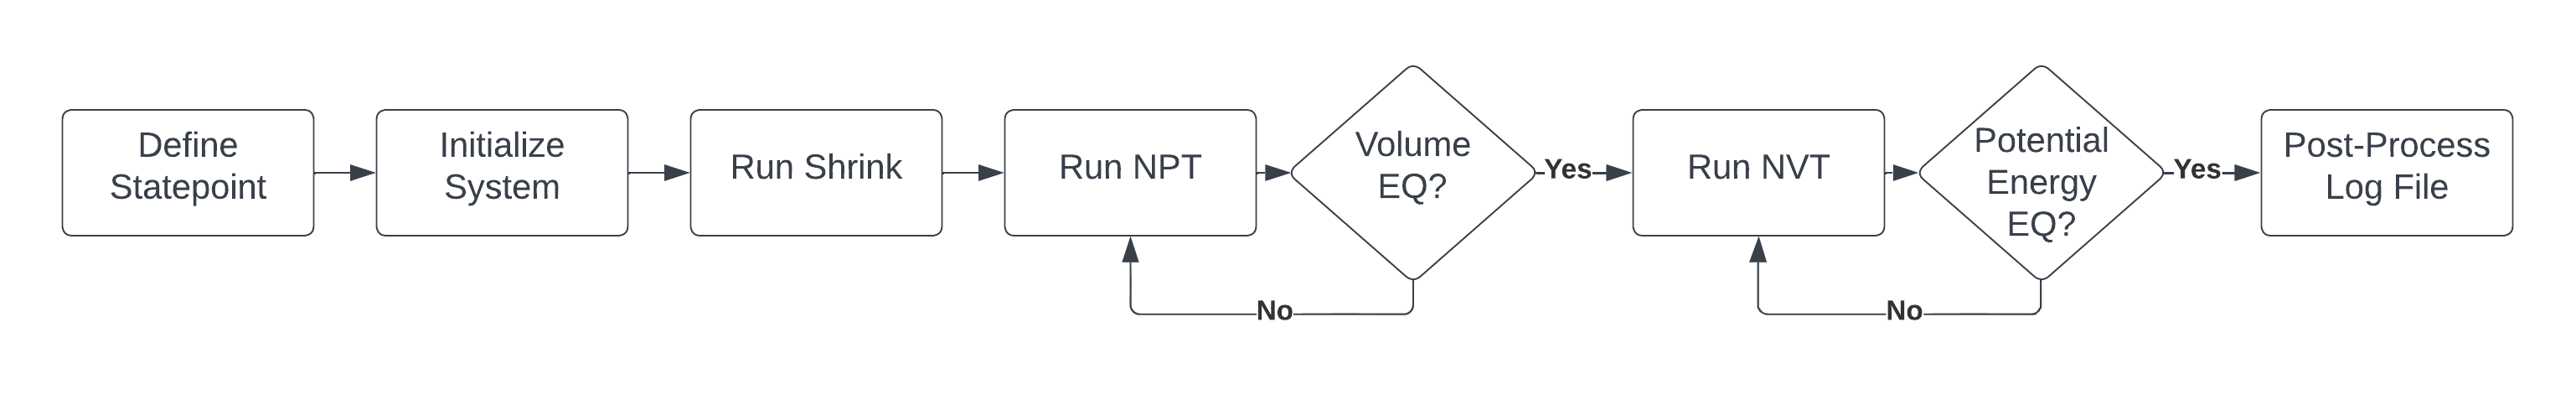
\includegraphics[width=\linewidth,keepaspectratio]{figures/rep_study/reproducibility_workflow.png}
    \caption{Workflow for HOOMD simulations in the reproducibility study.}\label{fig:rep_workflow}
\end{figure}
The workflow for the HOOMD simulations in shown in \autoref{fig:rep_workflow}. 
First the statepoint must be defined---this is handled by Signac \cite{Adorf2018, signac_zenodo, signac_scipy_2018, signac_scipy_2021}. 
The study is formatted as a Signac project, so all code---from system initialization to project analysis for all engines---is contained in a single repository.
The Signac project initialization script assigns all statepoint parameters (molecule, engine, replica, temperature, pressure, ensemble, N, box length, target density, mass, forcefield, cutoff style, long range correction, and $r_{cut}$) to each job. 
Then the system is initialized using that statepoint data. 
To ensure that all engines are starting with the same system, this process is generalized: All engines use the \lstinline{construct_system}, which wraps mBuild's \lstinline{fill_box} to creates an mBuild \lstinline{Compound} object containing the simulation box at the specified density populated with the specified number of molecules, and \lstinline{load_ff}, which loads the correct foyer \lstinline{Forcefield} object from the forcefield name in the statepoint. 
Then the forcefield is applied to the system box compound to generate a ParmEd structure\cite{Shirts2017}, where the atoms are typed according to the forcefield and and the relevant force parameters are also stored within the structure object. 
From there each engine takes the parameterized ParmEd structure and converts it to the necessary input format. 

For HOOMD this is done using the \lstinline{create_hoomd_forcefield} function in mBuild, which handles the unit scaling, initial snapshot creation, and neighborlist and force creation using the information stored in the ParmEd structure. 
Some adjustments are made to the snapshot and forcefield after this to handle rigid bodies, constrained bonds, neighborlist exclusions, and long range correction. 
The the simulation is initialized, the integrators, methods, and logging are set and the simulation can be run. 
The first run step in this process is to run a brief shrink step to bring the system to the desired density. 
The shrink step starts with the volume expanded by 8 times (each length of the target box is 2 times larger) then the box is shrunk in the NVT ensemble over 100 ps with a thermostat coupling value of 1 ps at the simulation temperature. 
The NPT run is initialized from the final frame of the shrink trajectory and is run at high thermostat (1 ps) and barostat (5 ps) coupling values initially (for the first 1 ns) to prevent large fluctuations in the pressure and kinetic temperature and then they are lowered (to 0.1 ps and 1 ps, respectively) for the duration of the run. %(Initial tau=1000dt tauS=5000dt for 1e6 steps then tauS=1000dt tau=100dt for 5e6 steps.) 

The NPT ensemble is run for a minimum of 6 ns, but after each NPT run, pymbar's \lstinline{detectEquilibration} function is used to check if the volume has equilibrated \cite{Chodera2007, Chodera2016, Shirts2008a}. 
If it has not, then the NPT simulation continues at the lower thermostat and barostat coupling values for an additional 5 ns. 
If the volume has equilibrated, then the statistically independent samples of the equilibrated volume are averaged and this average is logged to the job document and the job moves to the NVT run. 
The NVT run is initialized from the final frame of the NPT trajectory, but because this final frame may not be at the average volume, a short (20 ps) shrink period is done for the initial NVT run and then the simulation is run for 5 ns. 
After the NVT run, the same equilibration detection is used---this time looking at the potential energy values. If the potential energy is equilibrated, the NVT run is finished, otherwise it is run again for an additional 5 ns from the last frame of the proceeding NVT run. 
Finally the log file written out by HOOMD is processed to remove any extra headers within the data from restarted jobs, the pressure and temperature are converted from simulation units into kPa and K, and the density values are calculated from the volume and logged.

These scripts are publicly available on github \citep{reproducibility}.
The resulting output from all simulation engines is then converted to a standard format and unit system so that analysis can be done across simulation engines.
This data is then uploaded to a shared Dropbox folder using Rclone and once finalized the complete data will be distributed using Zenodo.

\section{Single point energy comparisons}

Single point energy calculations were added when discrepancies were found in the simulation results. 
With the benefit of hindsight, it is clear that starting with a single point energy comparison would've been much more efficient---allowing discovery of many issues early in the study. 
It is no doubt a good rule of thumb for simulators to provide a snapshot along with its energy breakdown when publishing. 
This data is very useful for those who attempt to replicate your work!

In order to determine the causes of discrepancies in the energies reported between engines, a single point energy evaluation was done for all systems. 
This involved distributing the complete information for the starting system: atom coordinates and bonding and box information. 
The reason this starting structure needed to be distributed is because it was necessary to ensure all starting structures were identical:
The packing functions in mBuild, including \lstinline{fill_box} which was used to create the initial simulation inputs for this study, are wrappers for PACKMOL \citep{Martinez2003, Martinez2009}.
PACKMOL uses an intrinsic random number generation method which is compiler dependent. 
The result is that PACKMOL creates different systems based on the operating system on which it was compiled.
In general, simulators are interested in comparing a sampling of the equilibrium ensemble, which should not depend on the initial position.
However, this discrepancy is important to note if one is trying to compare single point energies!
For this reason, it is good practice to distribute the input structure along with the code used to generate it.
This starting system was then initialized following the same procedure as the NPT/NVT ensemble simulations, but the simulation was not allowed to progress in time allowing direct comparison of the energies between engines.

Through the single point energy comparisons, we were able to determine that information about the 1-4 scaling and the combining rule were getting lost in the translation from foyer forcefield to ParmEd structure to engine input for Cassandra and Gromacs.
These errors were fixed by mbuild PR 1004 and 1010.
Initial comparison of the single point energies also showed large disagreement between the electrostatic energies of water in HOOMD and other engines. 
In HOOMD water was modelled as a rigid body. 
When the "rigid" neighborlist exclusion was added on to the default exclusions set by \lstinline{create_hoomd_forcefield} ("bond" and "1-3"), it was found that the exclusions were double counted by the PPPM energy calculation resulting in a large discrepancy in the electrostatic energy. 
This is now noted in HOOMD's documentation.

Choosing the correct parameters for the PPPM charge calculation---LAMMPS can set an error tolerance, but HOOMD sets the order and resolution and the error must be tuned using these parameters.

The single point energy values after applying the fixes discussed are included in \autoref{tab:sp_methane}-\autoref{tab:sp_ethanol}, and in general these values were found to agree with some noted discrepancies:
The long range and short range electrostatic energies may not be comparable between engines due to differences in the way these terms may be partitioned; however, the total electrostatic energy is comparable.

\section{Choosing a timestep}

For the ethanol system a smaller timestep was required.
When a timestep which was too large but small enough that the system didn't explode (i.e., the velocity update didn't push the particle outside of the simulation box) was used, the kinetic temperature was found to equilibrate to a lower value than was set in the NVT/NPT thermostat.
Unlike the other systems studied, ethanol has explicit hydrogens with harmonic bonds (water also has explicit hydrogens but it is rigid). 
Because hydrogen is such a light particle, the oscillations of bonds involving hydrogen are very fast.
The period of the harmonic bond is given by
\begin{equation}\label{eq:harmonic_period}
    T = \frac{2\pi}{\sqrt{\frac{k}{m}}}
\end{equation}
where k is the potential constant for that bond given in the forcefield and m is the mass of the particle.
Initially I was using a timestep of 0.001 (in simulation time units) while the period of the harmonic bond (see \autoref{eq:harmonic_period}) was 0.0118 (in simulation time units). \autoref{fig:harmonic_bond} shows the sensitivity of the harmonic bond sampling for different timesteps.
\begin{figure}[h!]
    \centering
    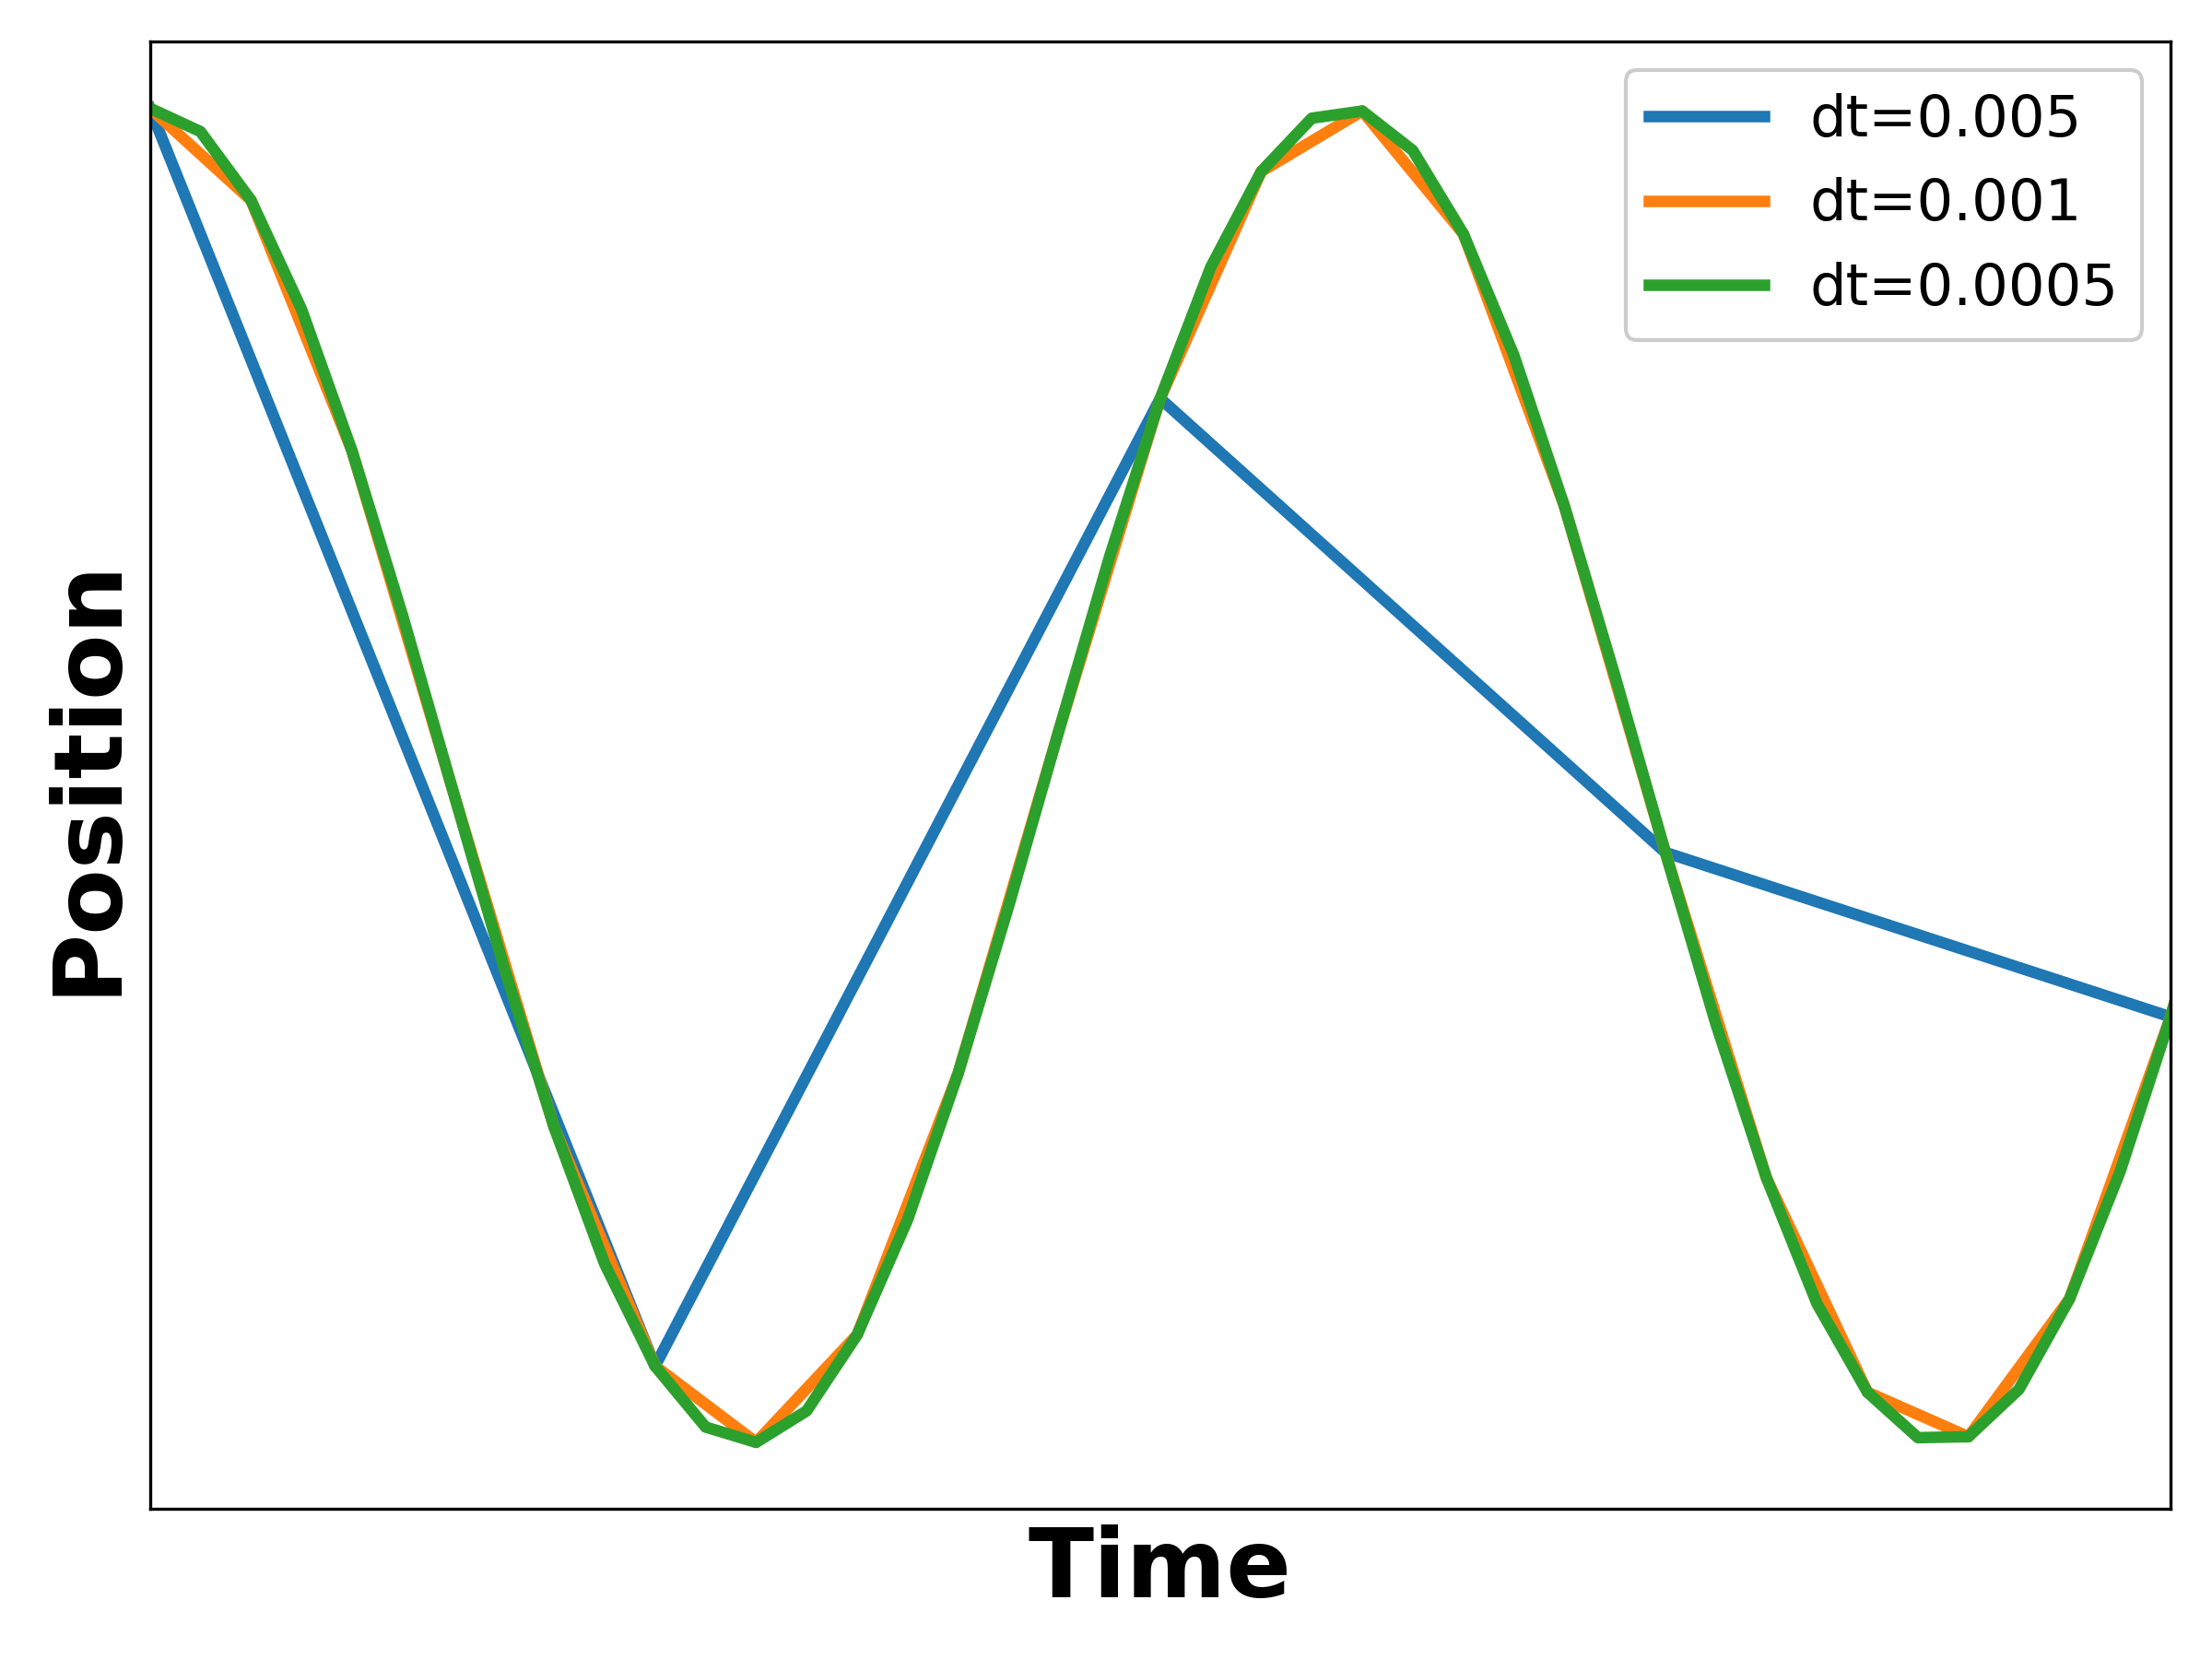
\includegraphics[width=0.8\linewidth,keepaspectratio]{figures/rep_study/harmonic_bond.png}
    \caption{Demonstration of how choosing too large a timestep can lead to poor sampling of the position of atoms in a harmonic bond. Note the divergence from sinusoidal as dt increases.}\label{fig:harmonic_bond}
\end{figure}
By using a smaller timestep (0.0005), the temperature equilibrated to the correct value.
\begin{figure}[h!]
    \centering
    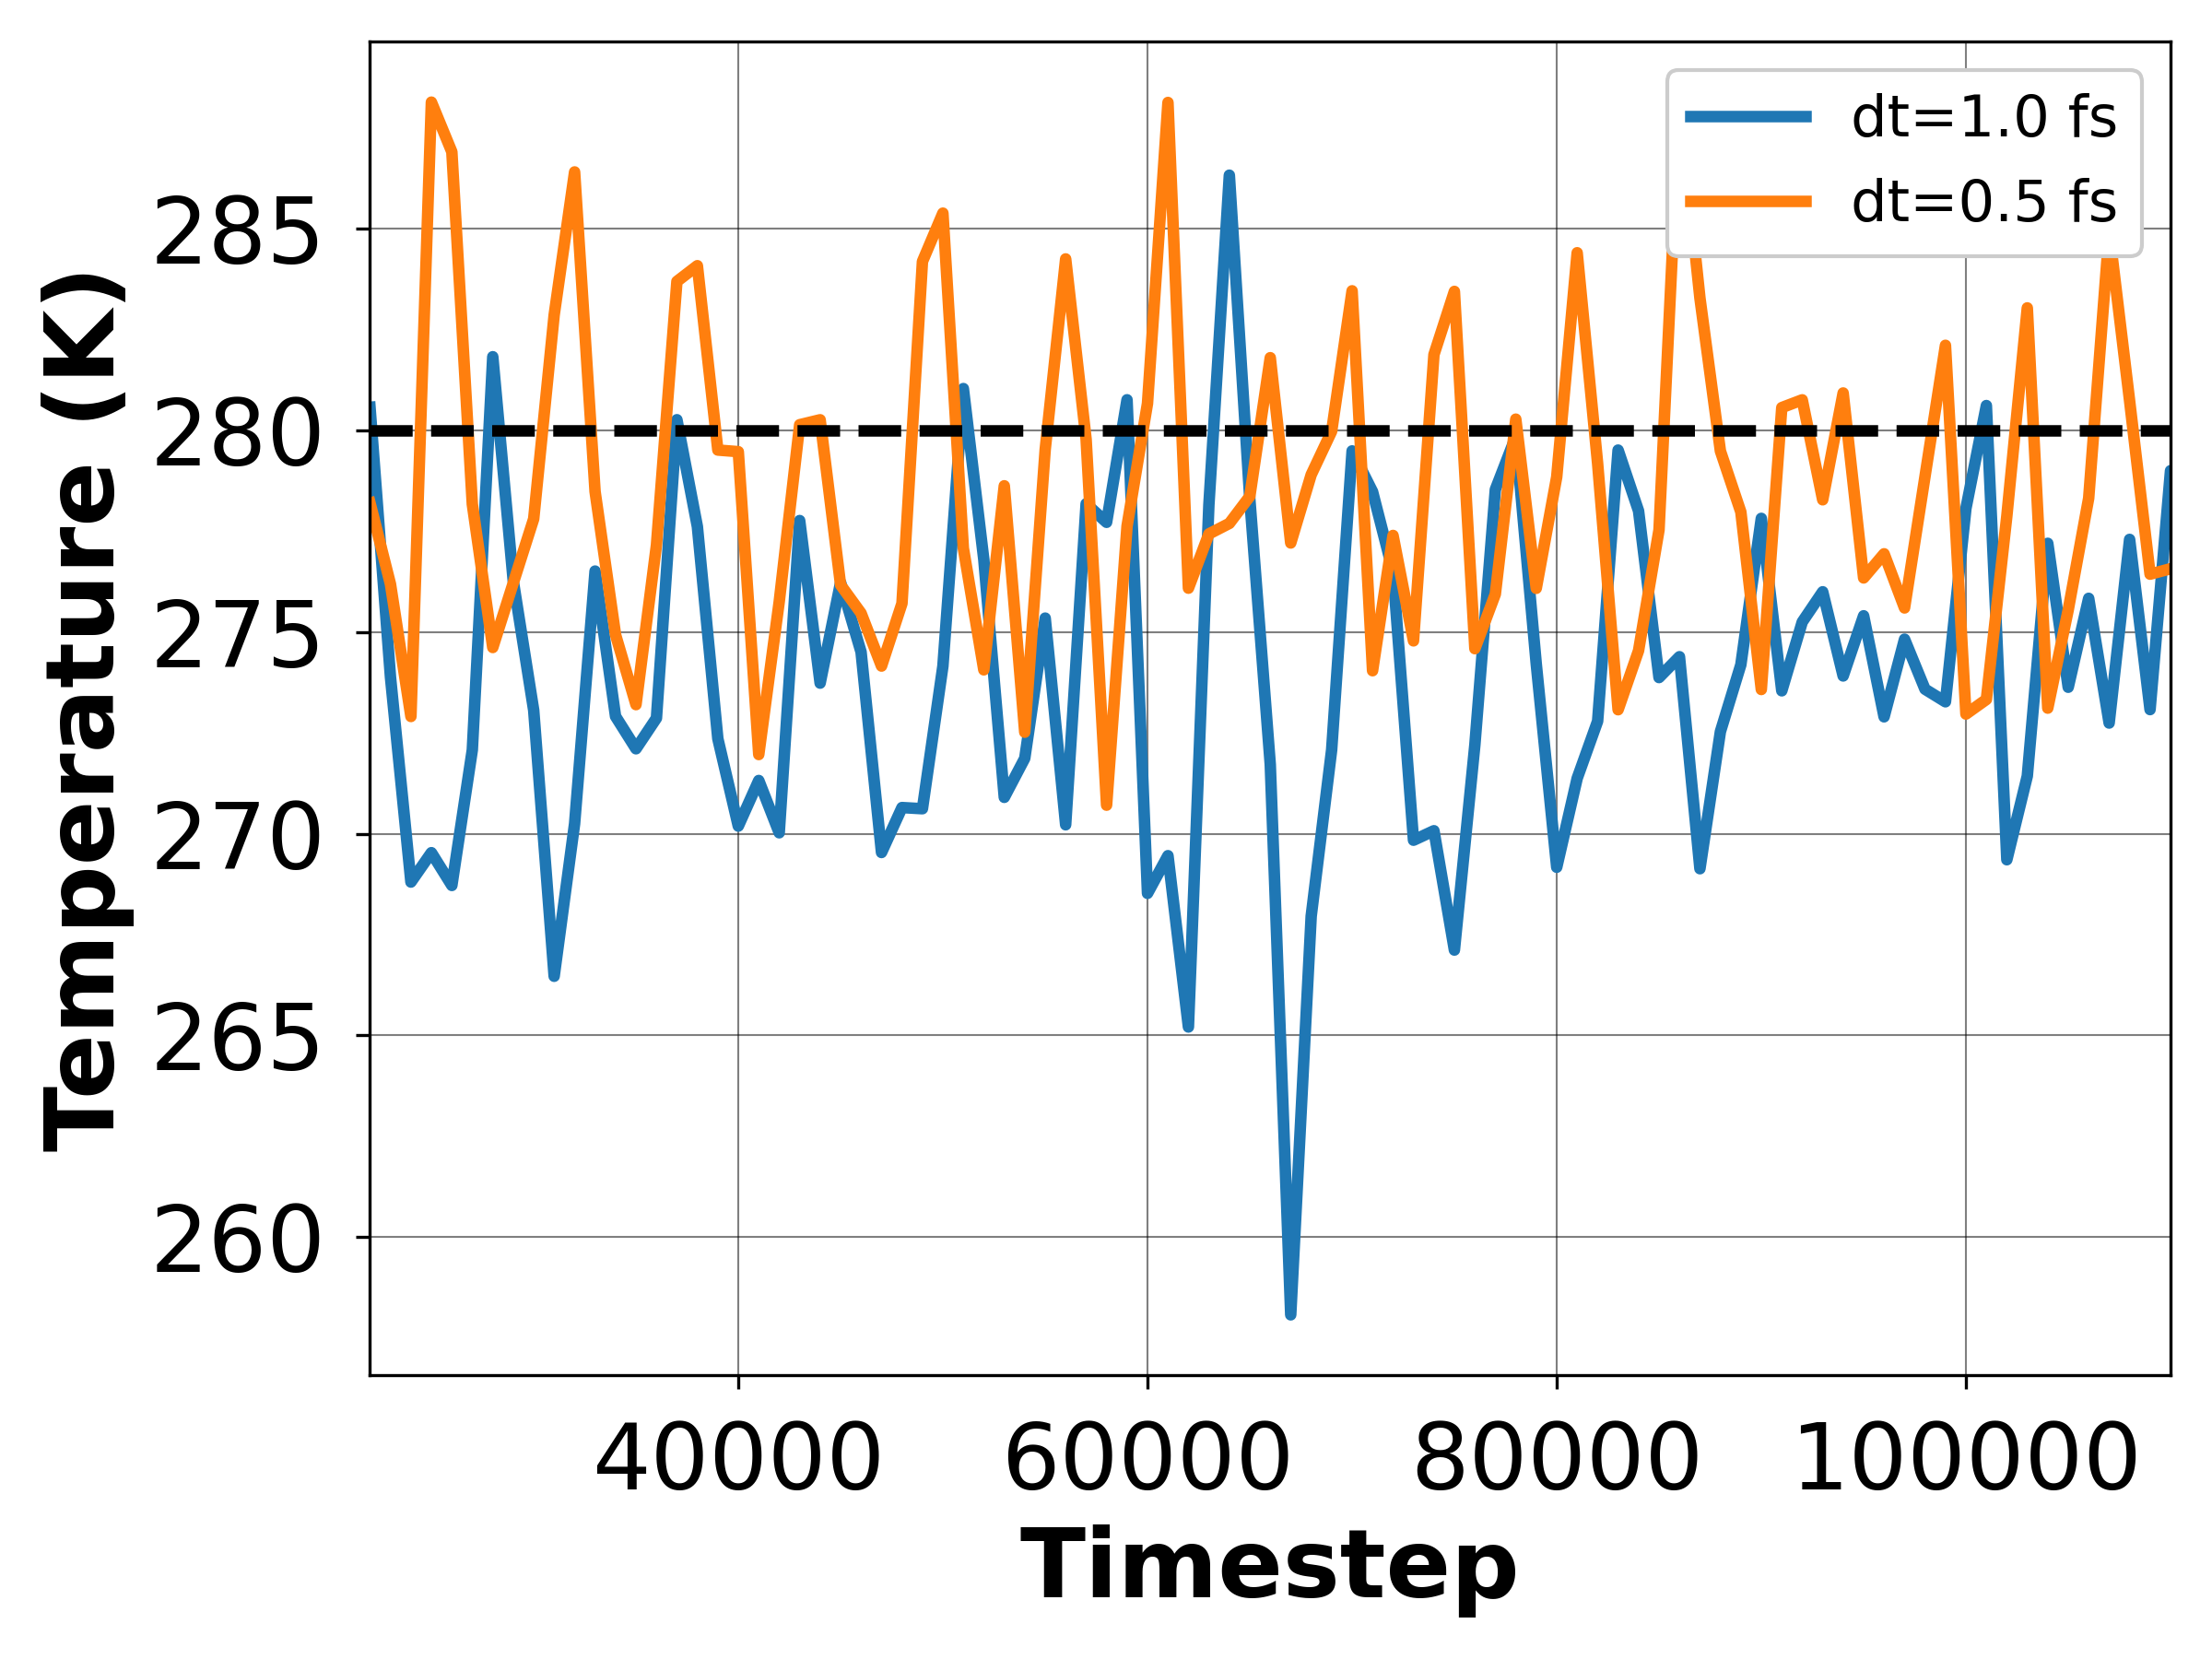
\includegraphics[width=0.8\linewidth,keepaspectratio]{figures/rep_study/temp_evolution.png}
    \caption{The evolution of temperature with time with the larger (1 fs) and a more reasonable (0.5 fs) timestep for the ethanol-AA system. The set temperature is shown as a dashed line. }\label{fig:temp_evo_ethanol}
\end{figure}
\autoref{fig:temp_evo_ethanol} and \autoref{fig:temp_evo_methane} show the sensitivity of the equilibrium temperature to timestep based on system complexity. Both plots are very noisy because they show only the initial 100 ps post-shrink equilibration in the NVT ensemble, however the methane temperature fluctuates around the set value and these fluctuations are small (only a couple of degrees K) and smooth. While the ethanol fluctuations are much larger, and with the larger timestep, the fluctuations are not about the set equilibrium temperature.
\begin{figure}[h!]
    \centering
    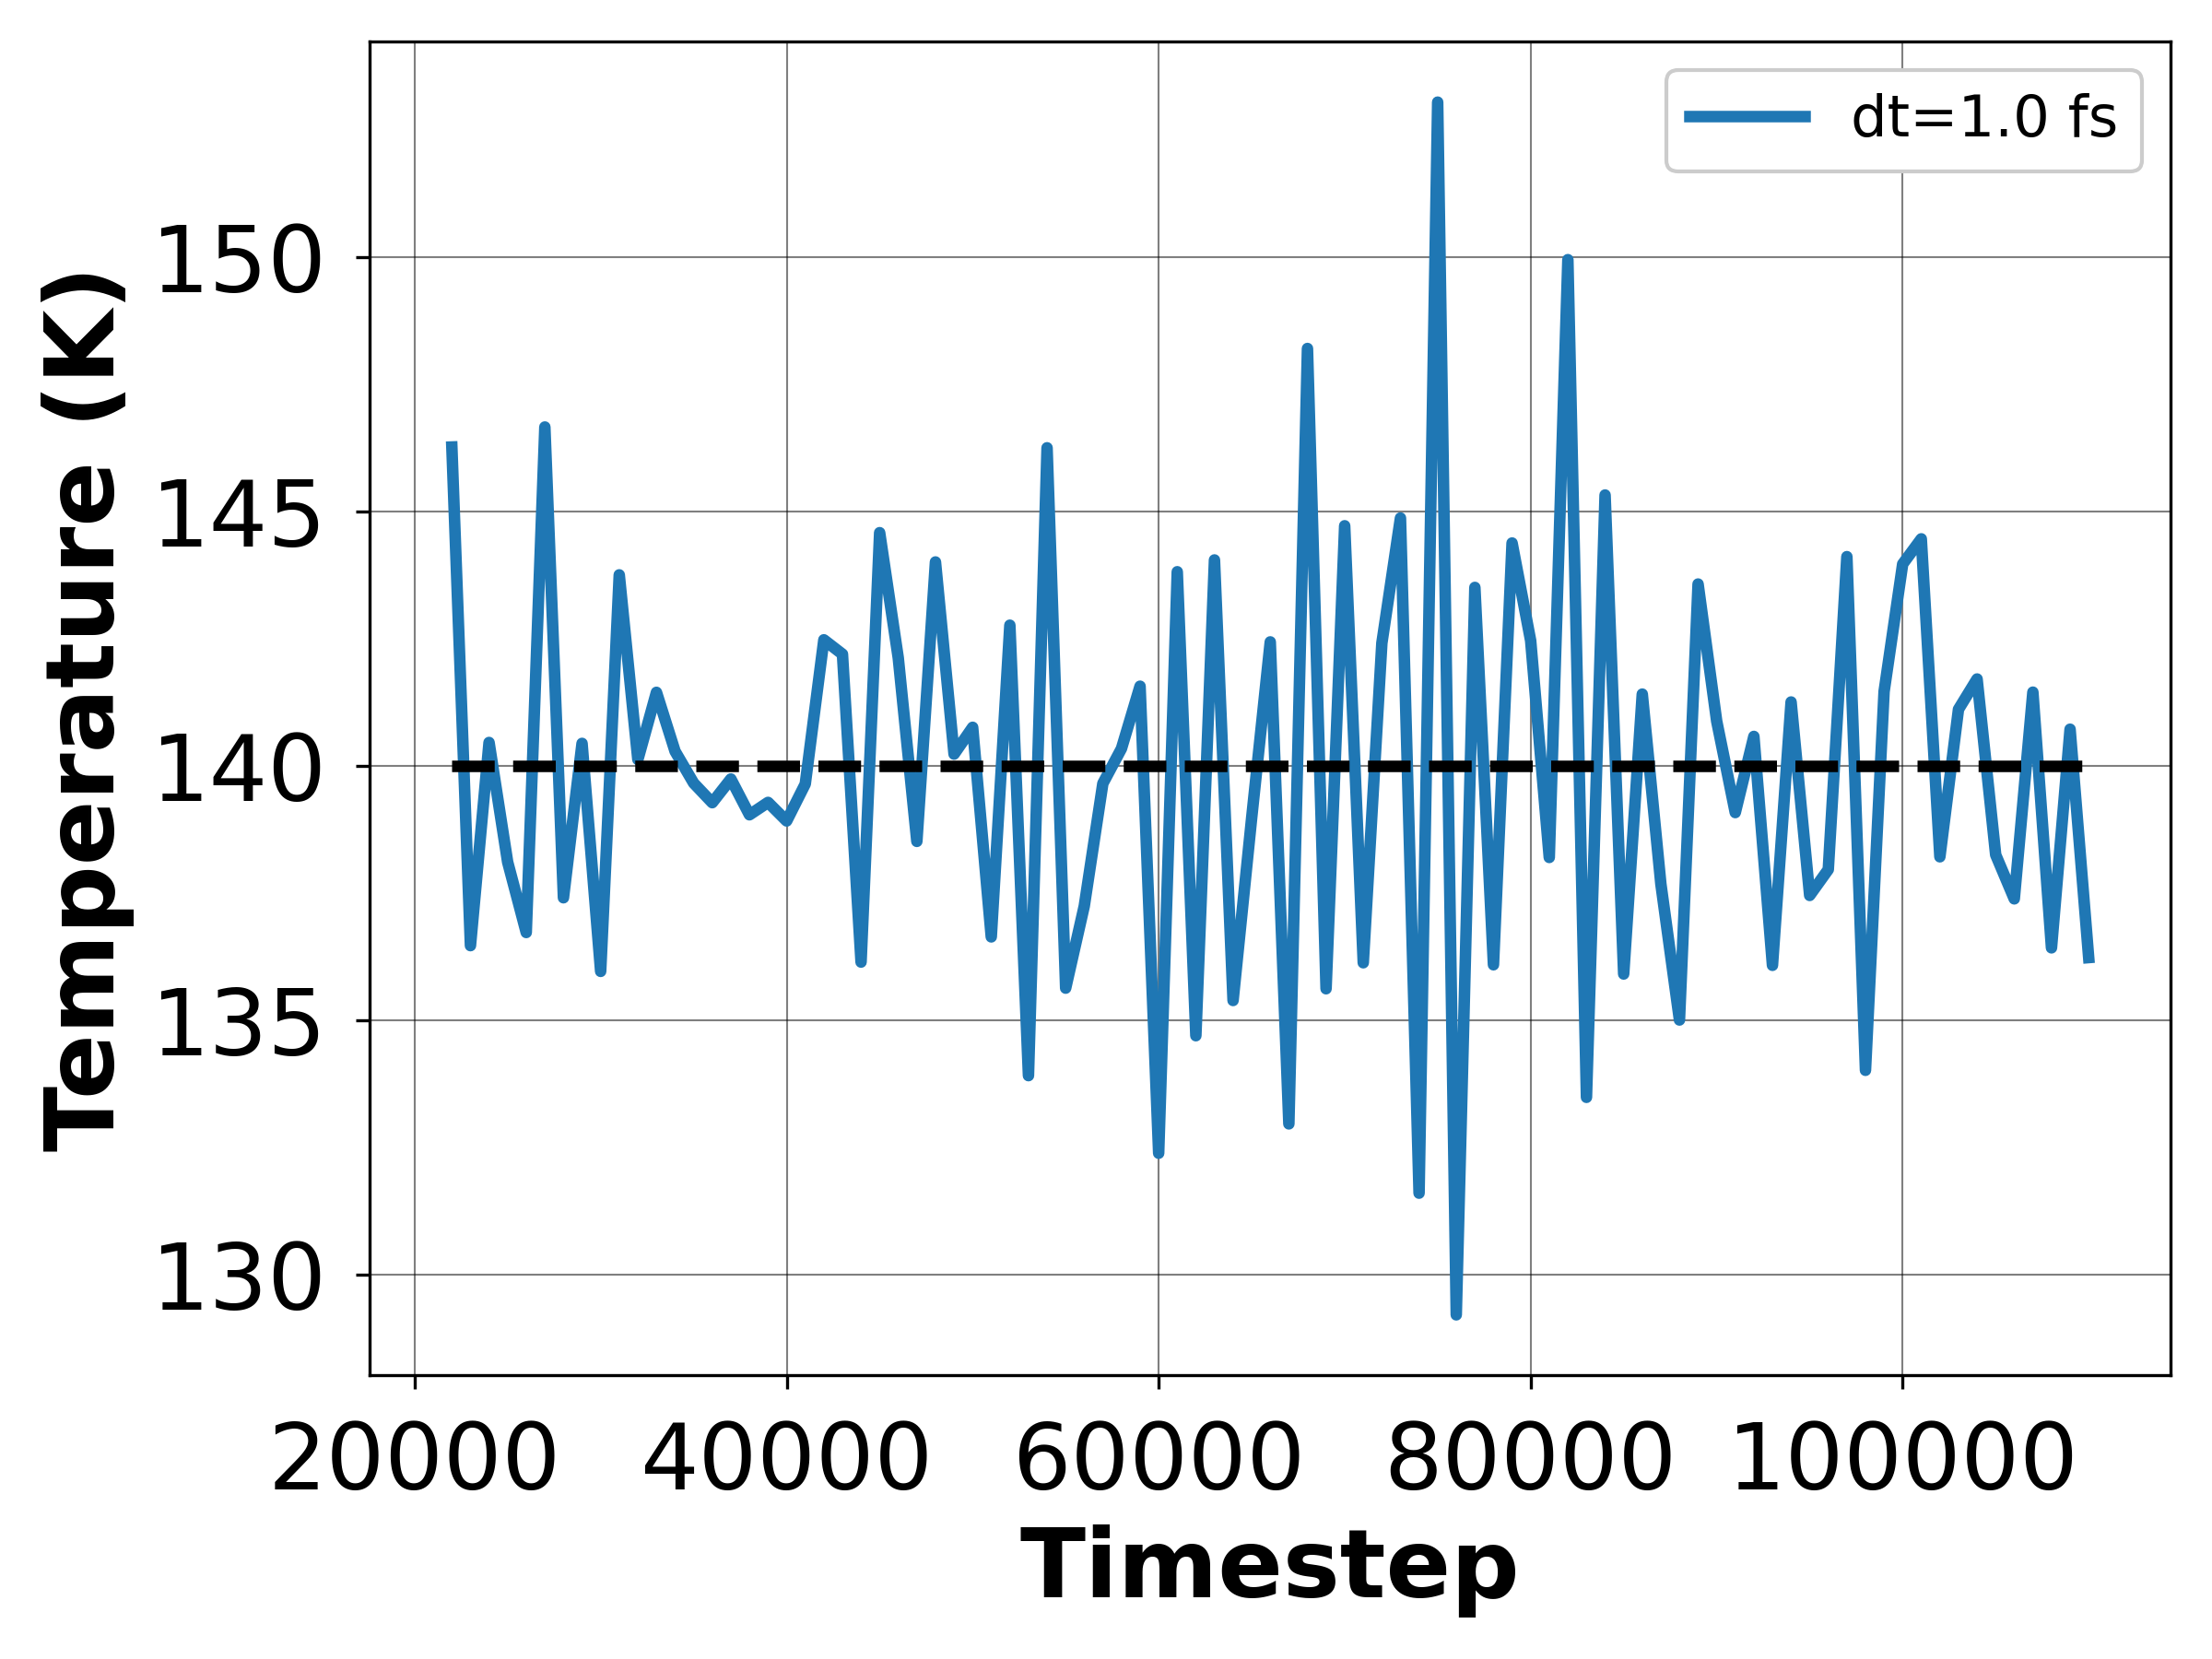
\includegraphics[width=0.8\linewidth,keepaspectratio]{figures/rep_study/temp_evolution_methane.png}
    \caption{The evolution of temperature with time with the larger (1 fs) timestep for the methane-UA system. The set temperature is shown as a dashed line.}\label{fig:temp_evo_methane}
\end{figure}
%% why did it appear to equilibrate though?

\subsection{Cutoff schemes}\label{sec:cutoff}

In order to correct for the contributions of interactions beyond the cutoff, isotropic integrated long range tail corrections were applied to the Lennard-Jones pair potentials. The pressure and energy corrections $\Delta P$ and $\Delta E$ are given by
\begin{equation}\label{lrc_p}
    \Delta P = \frac{-2\pi}{3} \sum_{i=1}^{n} \rho_i \sum_{j=1}^{n} \rho_j
    \int_{r_\mathrm{cut}}^{\infty} \left( r
    \frac{\mathrm{d}V_{ij}(r)}{\mathrm{d}r} \right) r^2 \,\,\mathrm{d}r  
\end{equation}
and
\begin{equation}\label{lrc_e}
    \Delta E = 2\pi \sum_{i=1}^{n} N_i \sum_{j=1}^{n} \rho_j
    \int_{r_\mathrm{cut}}^{\infty} V_{ij}(r) r^2\,\,\mathrm{d}r, 
\end{equation}
where $n$ is the number of unique particle types in the system, $\rho_{i}$ is the number density of particles of type $i$ in the system, $V_{ij}(r)$ is the pair potential between particles of type $i$ and $j$, and $N_{i}$ is the number of particles of type $i$ in the system. These expressions assume that the radial pair distribution functions, $g_{ij}(r)$, are unity at the cutoff and beyond. code referencing the formulas in Frenkel and Smit \citep{frenkel2001understanding} and from eq 5 of  \citep{Sun1998}. see Equation~\eqref{lrc_p}, \eqref{lrc_e}

If a hard cutoff was used, the density did not agree between the MD and MC methods.
Some MC engines use impulsive contribution to the pressure which is not accounted for in MD and this may have some effect \citep{frenkel2001understanding}.
However GOMC does not have impulsive correction but has agreement with MC3S. Why do we see consistency between MD? and MC?
This is due to innate differences in the two methods: MD is using the interparticle forces---the derivative of the potential w.r.t. r---while MC uses the potential values outright.
Due to the discontinuity in the potential with hard cutoff, the force will be infinite in MD.

When using the shifted cutoff we may see similar discrepancies between the two methods. 
The potential is no longer discontinuous, but has an inflection point at $r_{cut}$ so the force will be discontinuous but not infinite.
Shifted cutoff is also not ideal for the force-fields we are using as they were all parameterized with LRC. 

So in order to achieve agreement between methods, we needed to use LRC to energy and pressure. 
By using the energy-pressure correction, we were able to get agreement between the energies and densities of both methods. 
Slight differences in the pressures were noted depending on if the ideal gas approximation is used for the pressure calculation.
Pressure is not matching between engines for the single snapshot of methane. 
The difference is due to the ideal gas contribution to pressure. 
Some engines are calculating the pressure at 0K and others at the specified temperature.
In order to assess the impact of the cut off scheme, a substudy was performed examining the effect of only cutoff on the simplest system, united atom methane. This system is uncharged and contains a single, unbonded particle type, so it only has Lennard-Jones type interactions. When a hard cutoff is used (see \autoref{fig:hard_cutoff}), there is a large discrepancy between the MD engines (GROMACS, LAMMPS, and HOOMD) and the MC engines (GOMC, Cassandra, and MCCCS). 
\begin{figure}[h!]
    \centering
    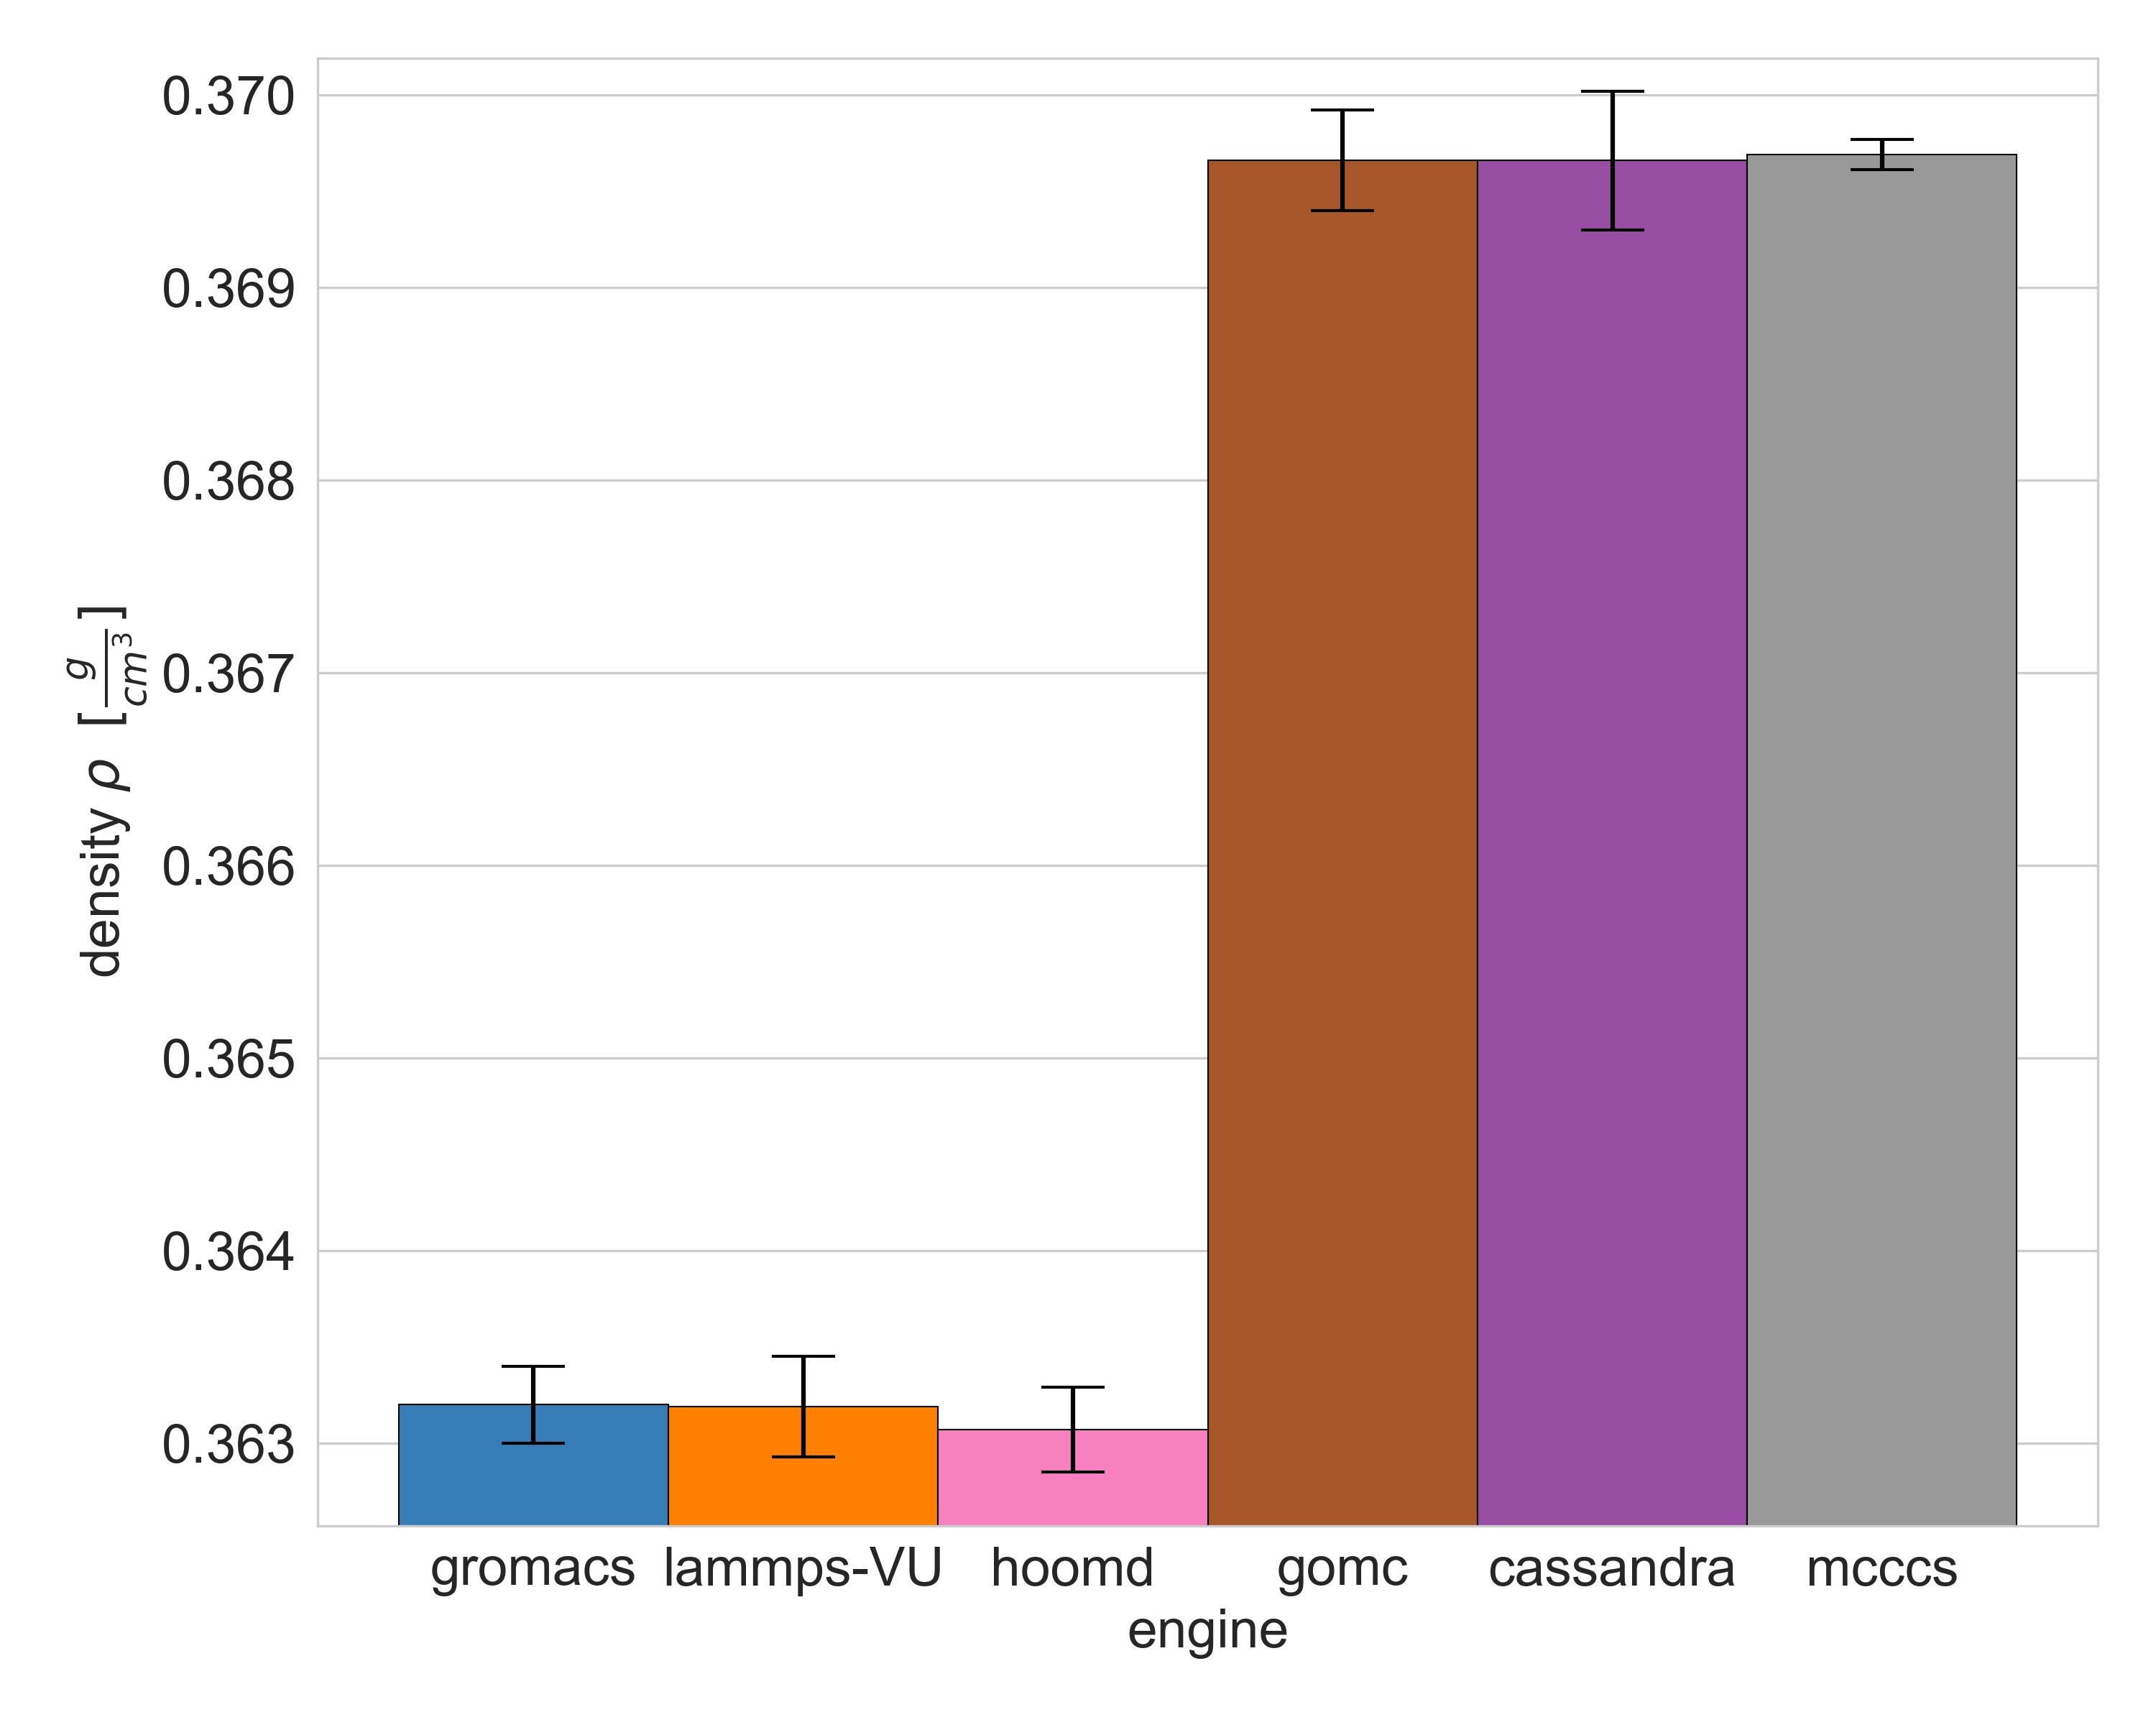
\includegraphics[width=0.8\linewidth,keepaspectratio]{figures/rep_study/hard_cutoff.png}
    \caption{Average density from NPT simulation of methane using "hard" cutoff by engine. Average of independent samples from equilibrated regions of 16 replicates. Error bars represent two standard deviations.}\label{fig:hard_cutoff}
\end{figure}
When a shifted cutoff is used (see \autoref{fig:shift_cutoff}), all engines equilibrate to the same density within error, but the density is much lower than the predicted value---the density of methane at 140K and 1318kPa should be 0.37808 g/cm$^3$\cite{NISTwebbook}.
\begin{figure}[h!]
    \centering
    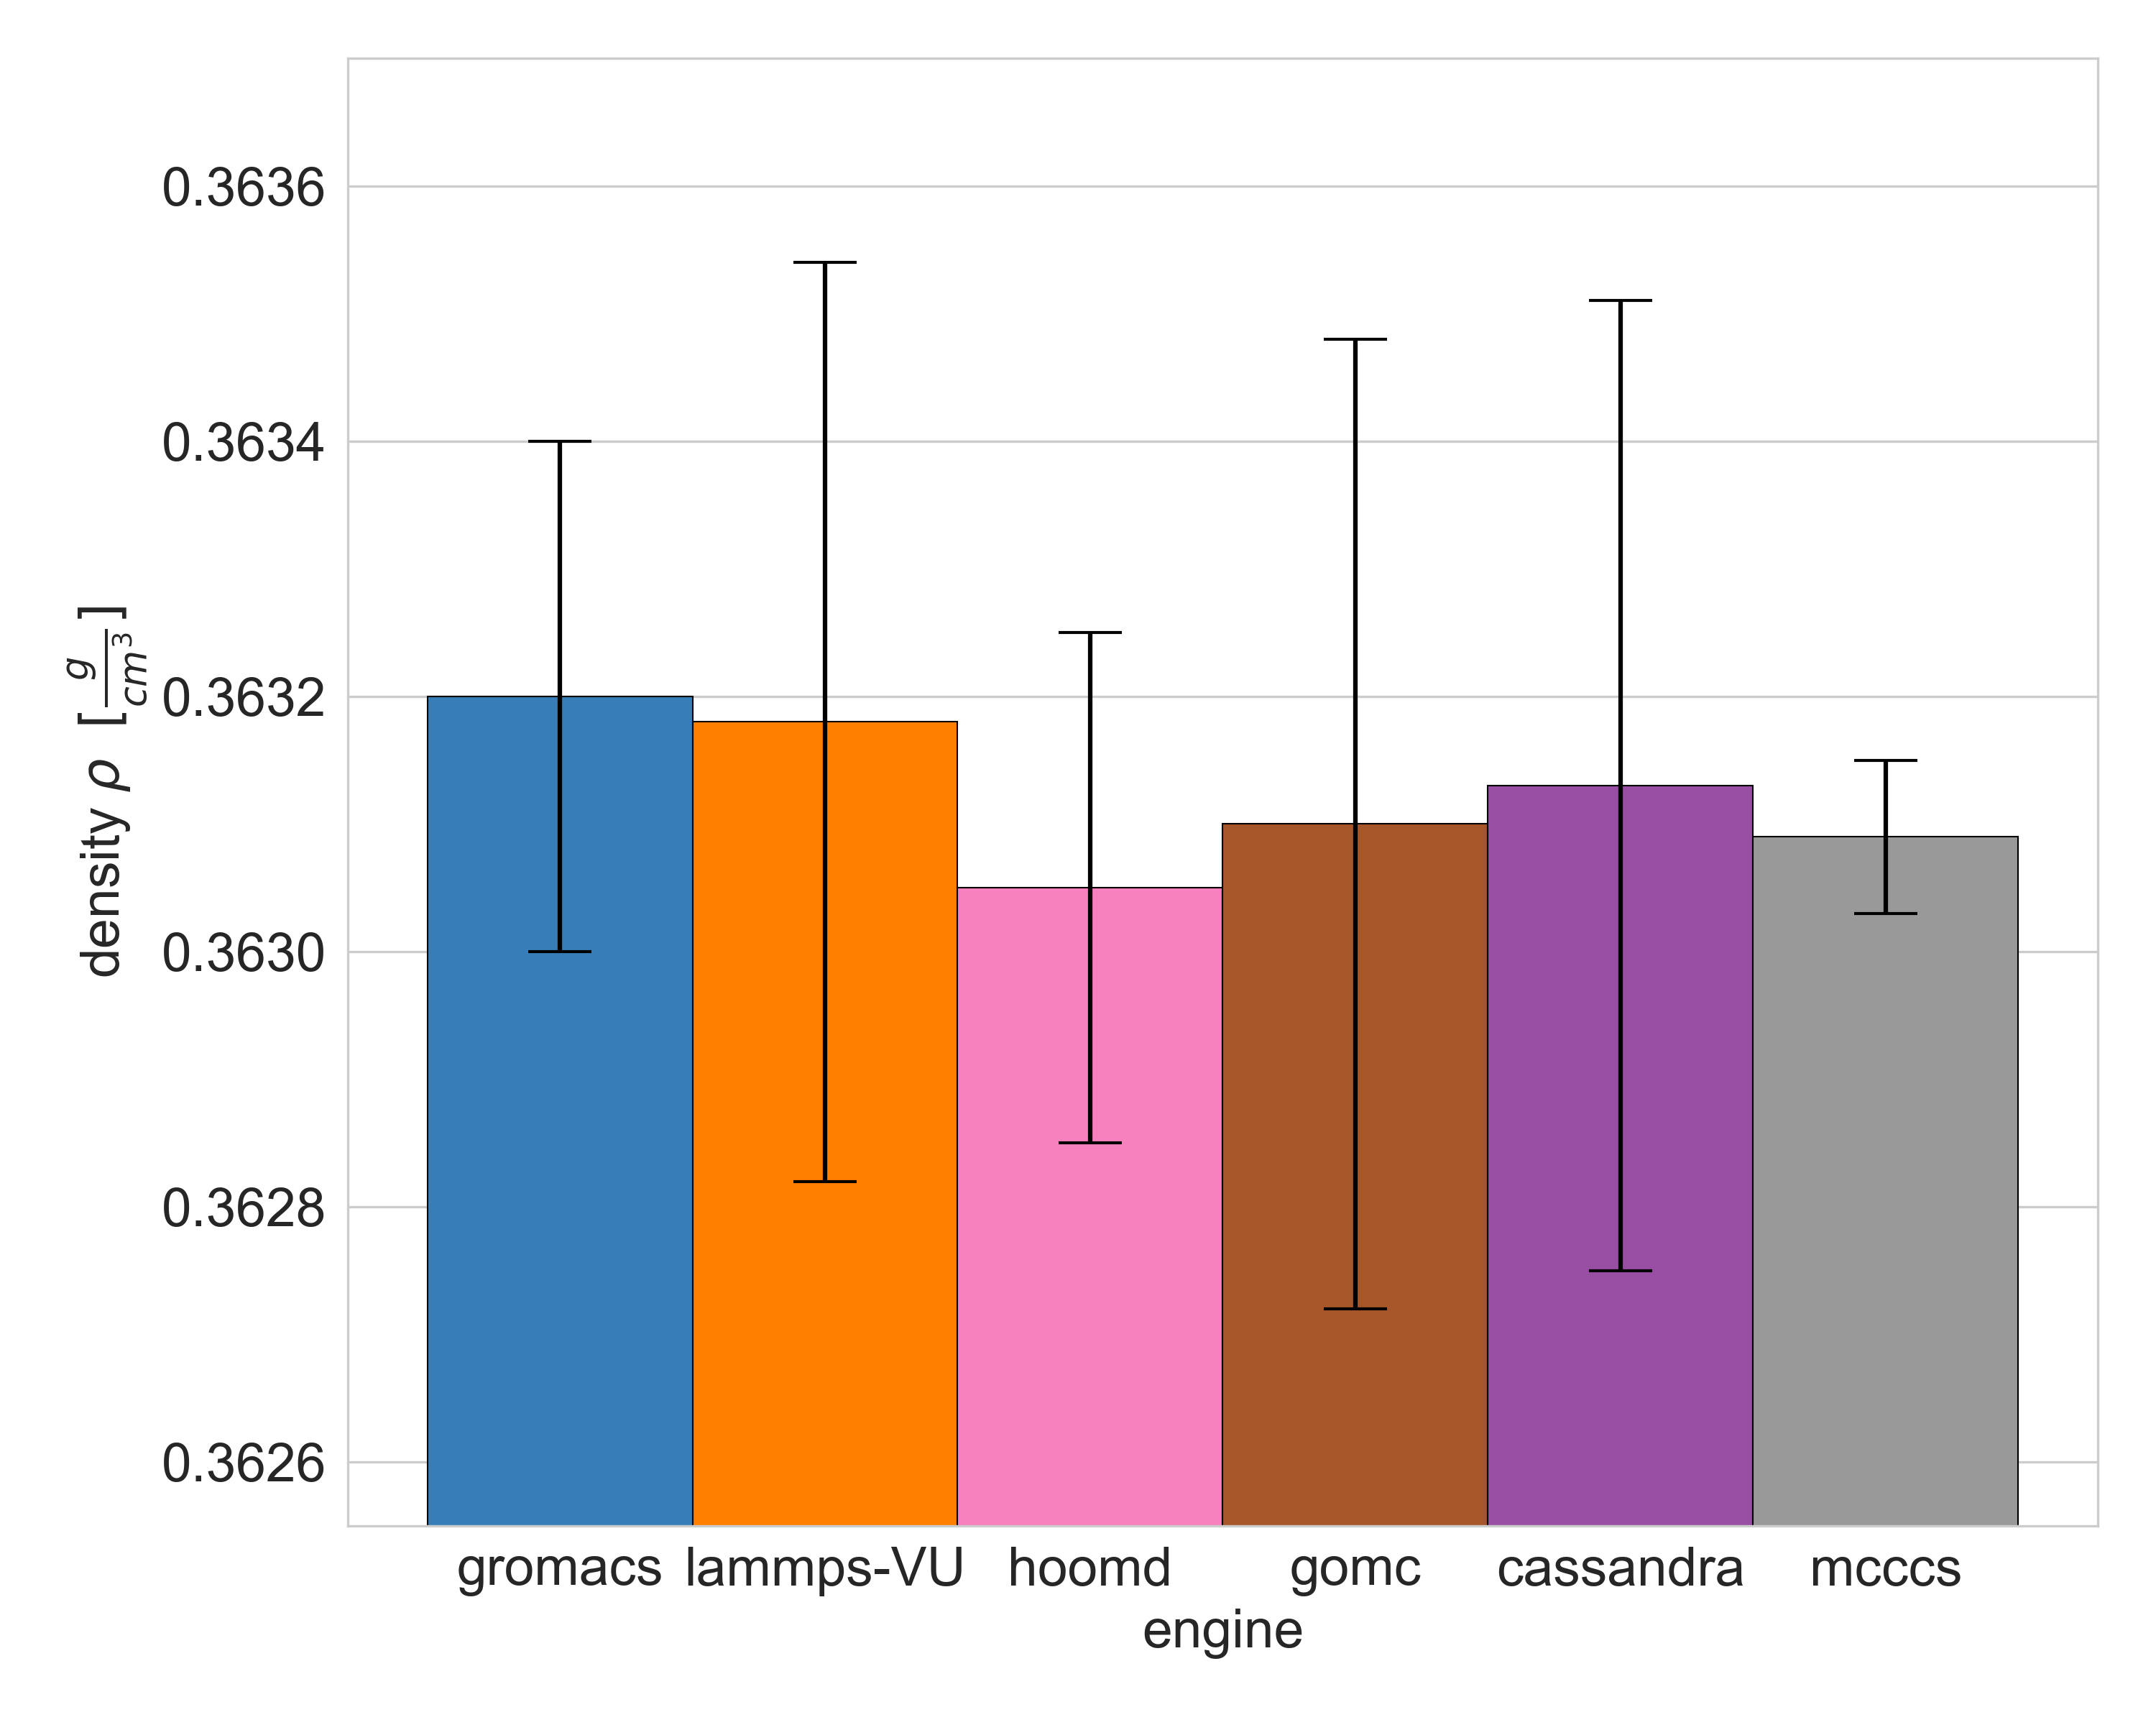
\includegraphics[width=0.8\linewidth,keepaspectratio]{figures/rep_study/shift_cutoff.png}
    \caption{Average density from NPT simulation of methane using "shifted" cutoff by engine. Average of independent samples from equilibrated regions of 16 replicates. Error bars represent two standard deviations.}\label{fig:shift_cutoff}
\end{figure}
So in order to get agreement between engines and closer to the correct density value, the correction to the energy and pressure was needed (see \autoref{fig:lrc_cutoff}).
\begin{figure}[h!]
    \centering
    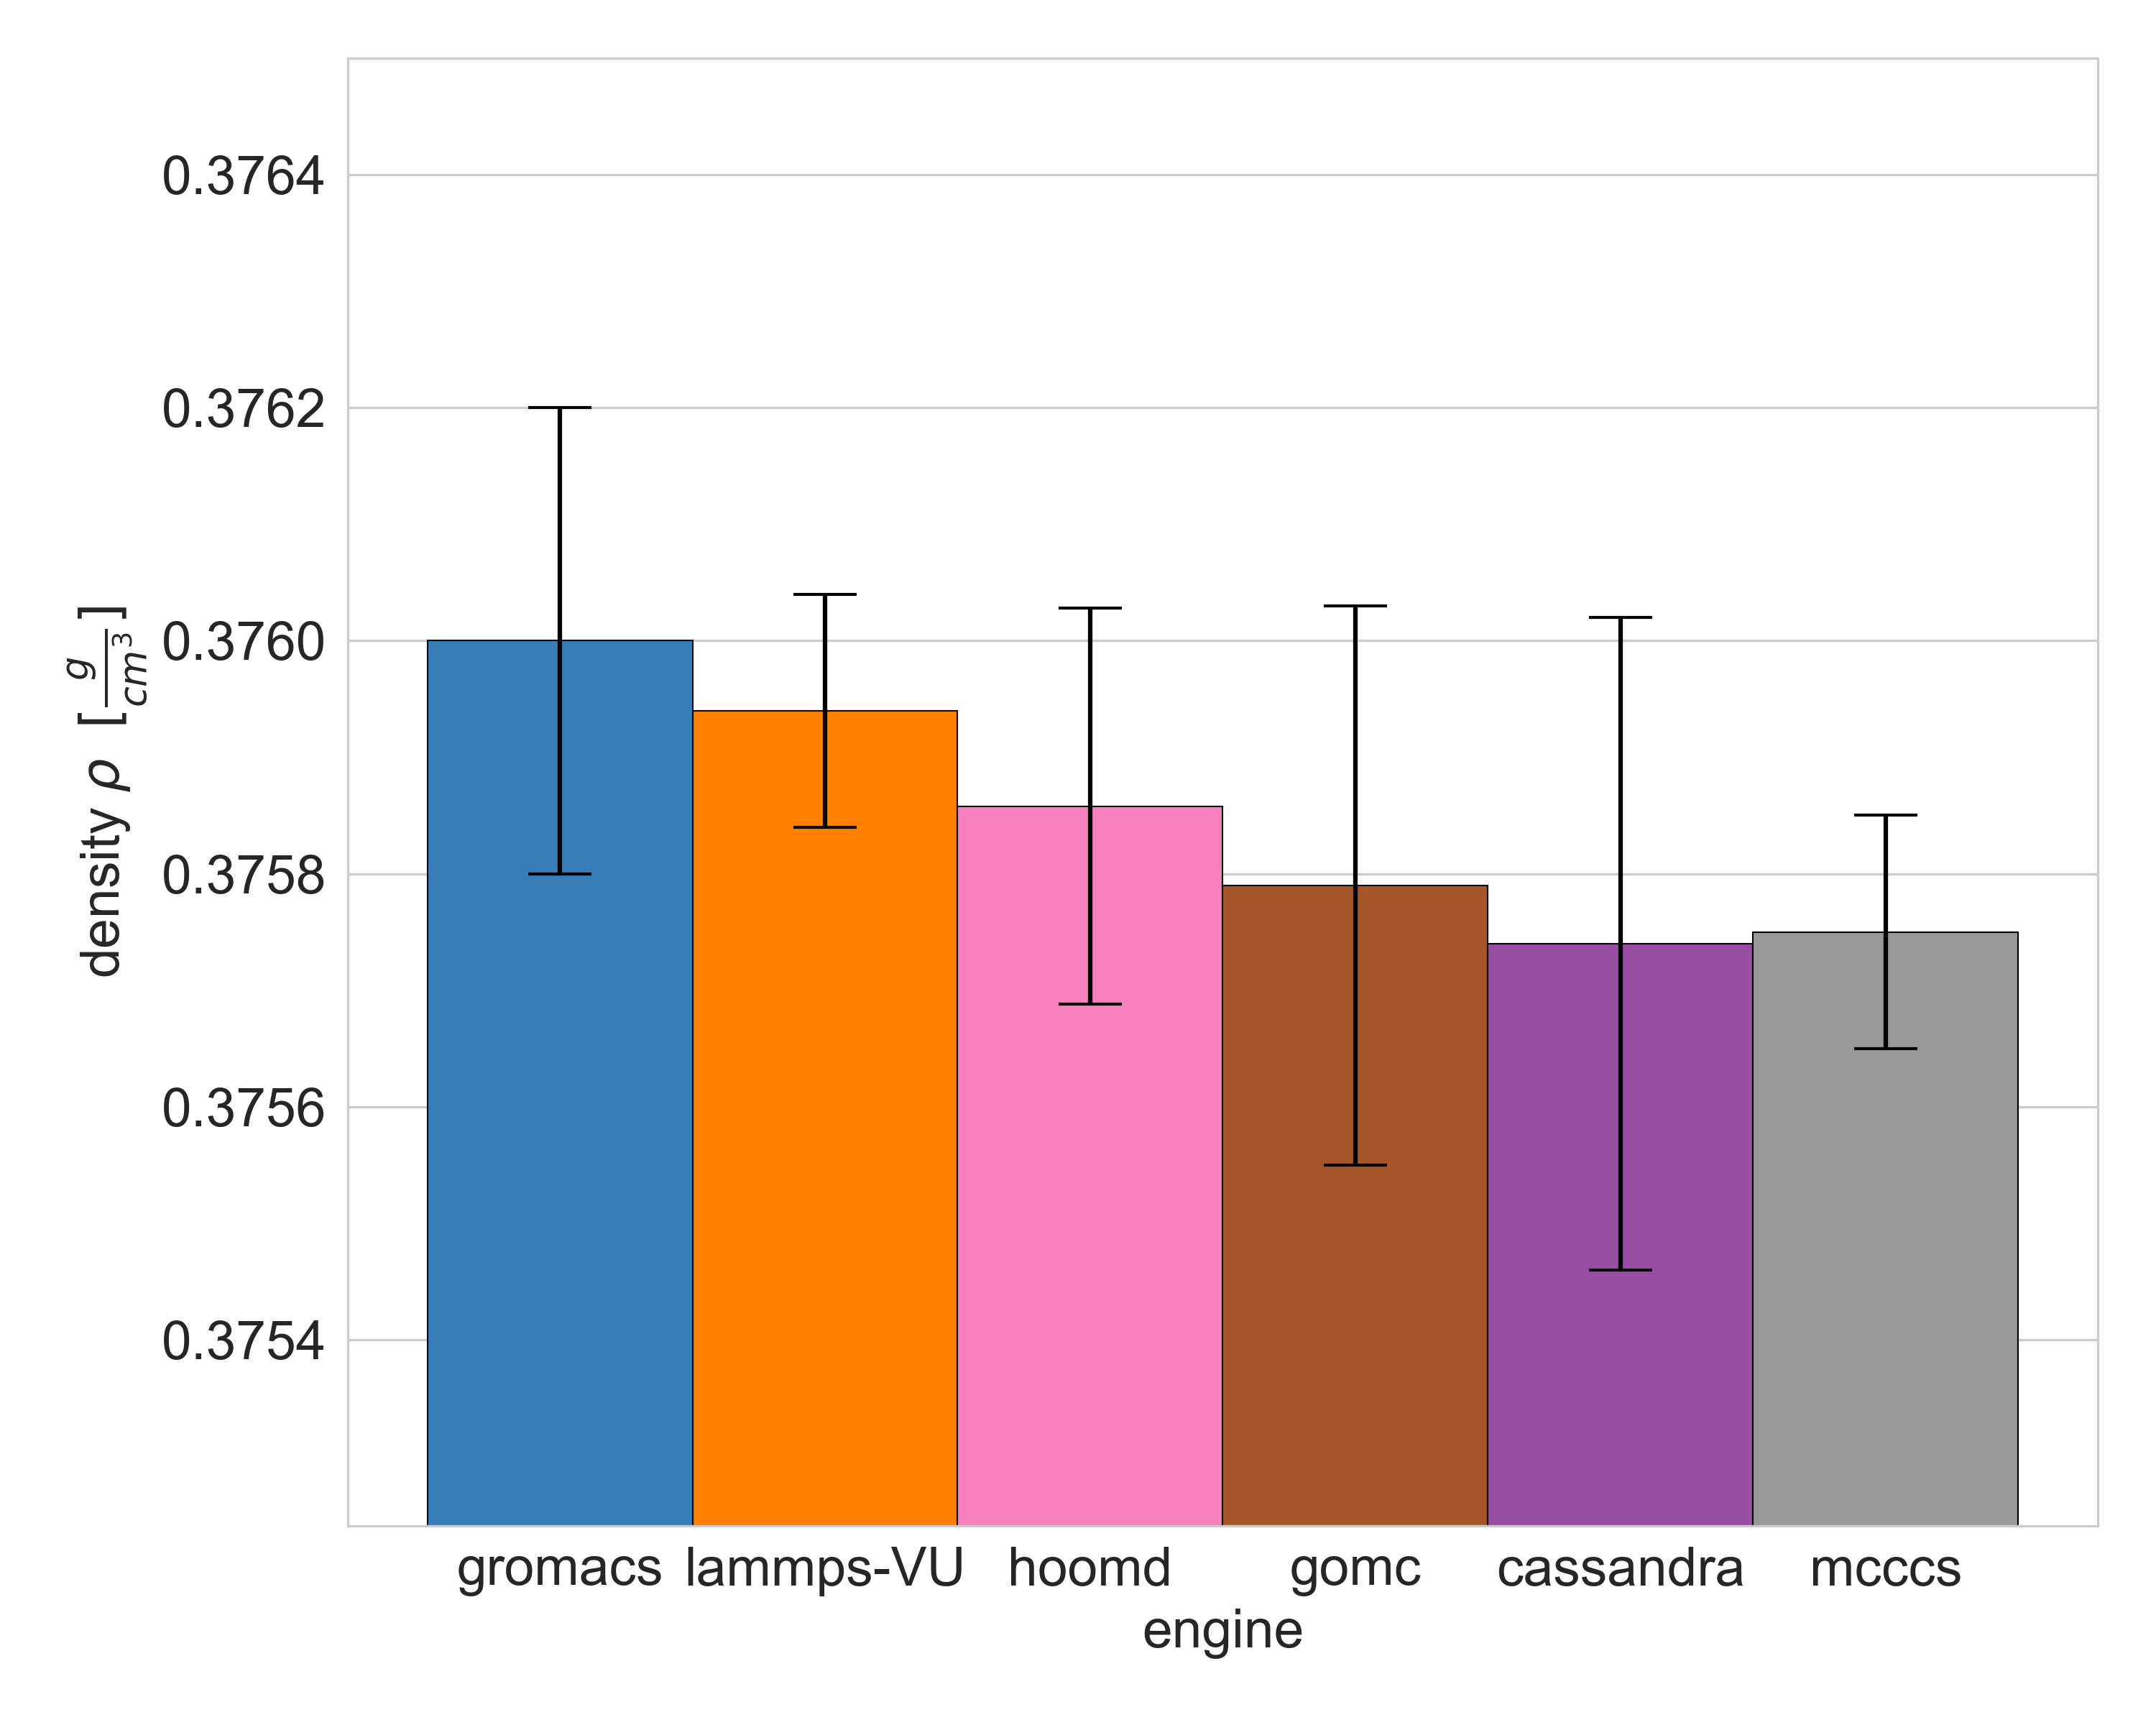
\includegraphics[width=0.8\linewidth,keepaspectratio]{figures/rep_study/lrc_cutoff.png}
    \caption{Average density from NPT simulation of methane using energy and pressure long range correction by engine. Average of independent samples from equilibrated regions of 16 replicates. Error bars represent two standard deviations.}\label{fig:lrc_cutoff}
\end{figure}

\subsection{Rigid constraints}

I also contributed to the code which calculates rigid bodies in HOOMD v3 % cite my PR?
HOOMD has some idiosyncrasies with its handling of rigid bodies: body particles must be first in the snapshot and the bodies must all have the same orientation on initialization. To reduce the cognitive load for users, HOOMD recommends creating the body constituent particles using the create\_bodies function, but this conflicts with using the MoSDeF initialization.

\section{Results} 

%% here we'll want to show off the <PE> and <Density> values before and after your software fixes and maybe point to particular commits/PRs.
analysis metrics: energy, density, RDF, MSD

\begin{figure}[h!]
    \centering
    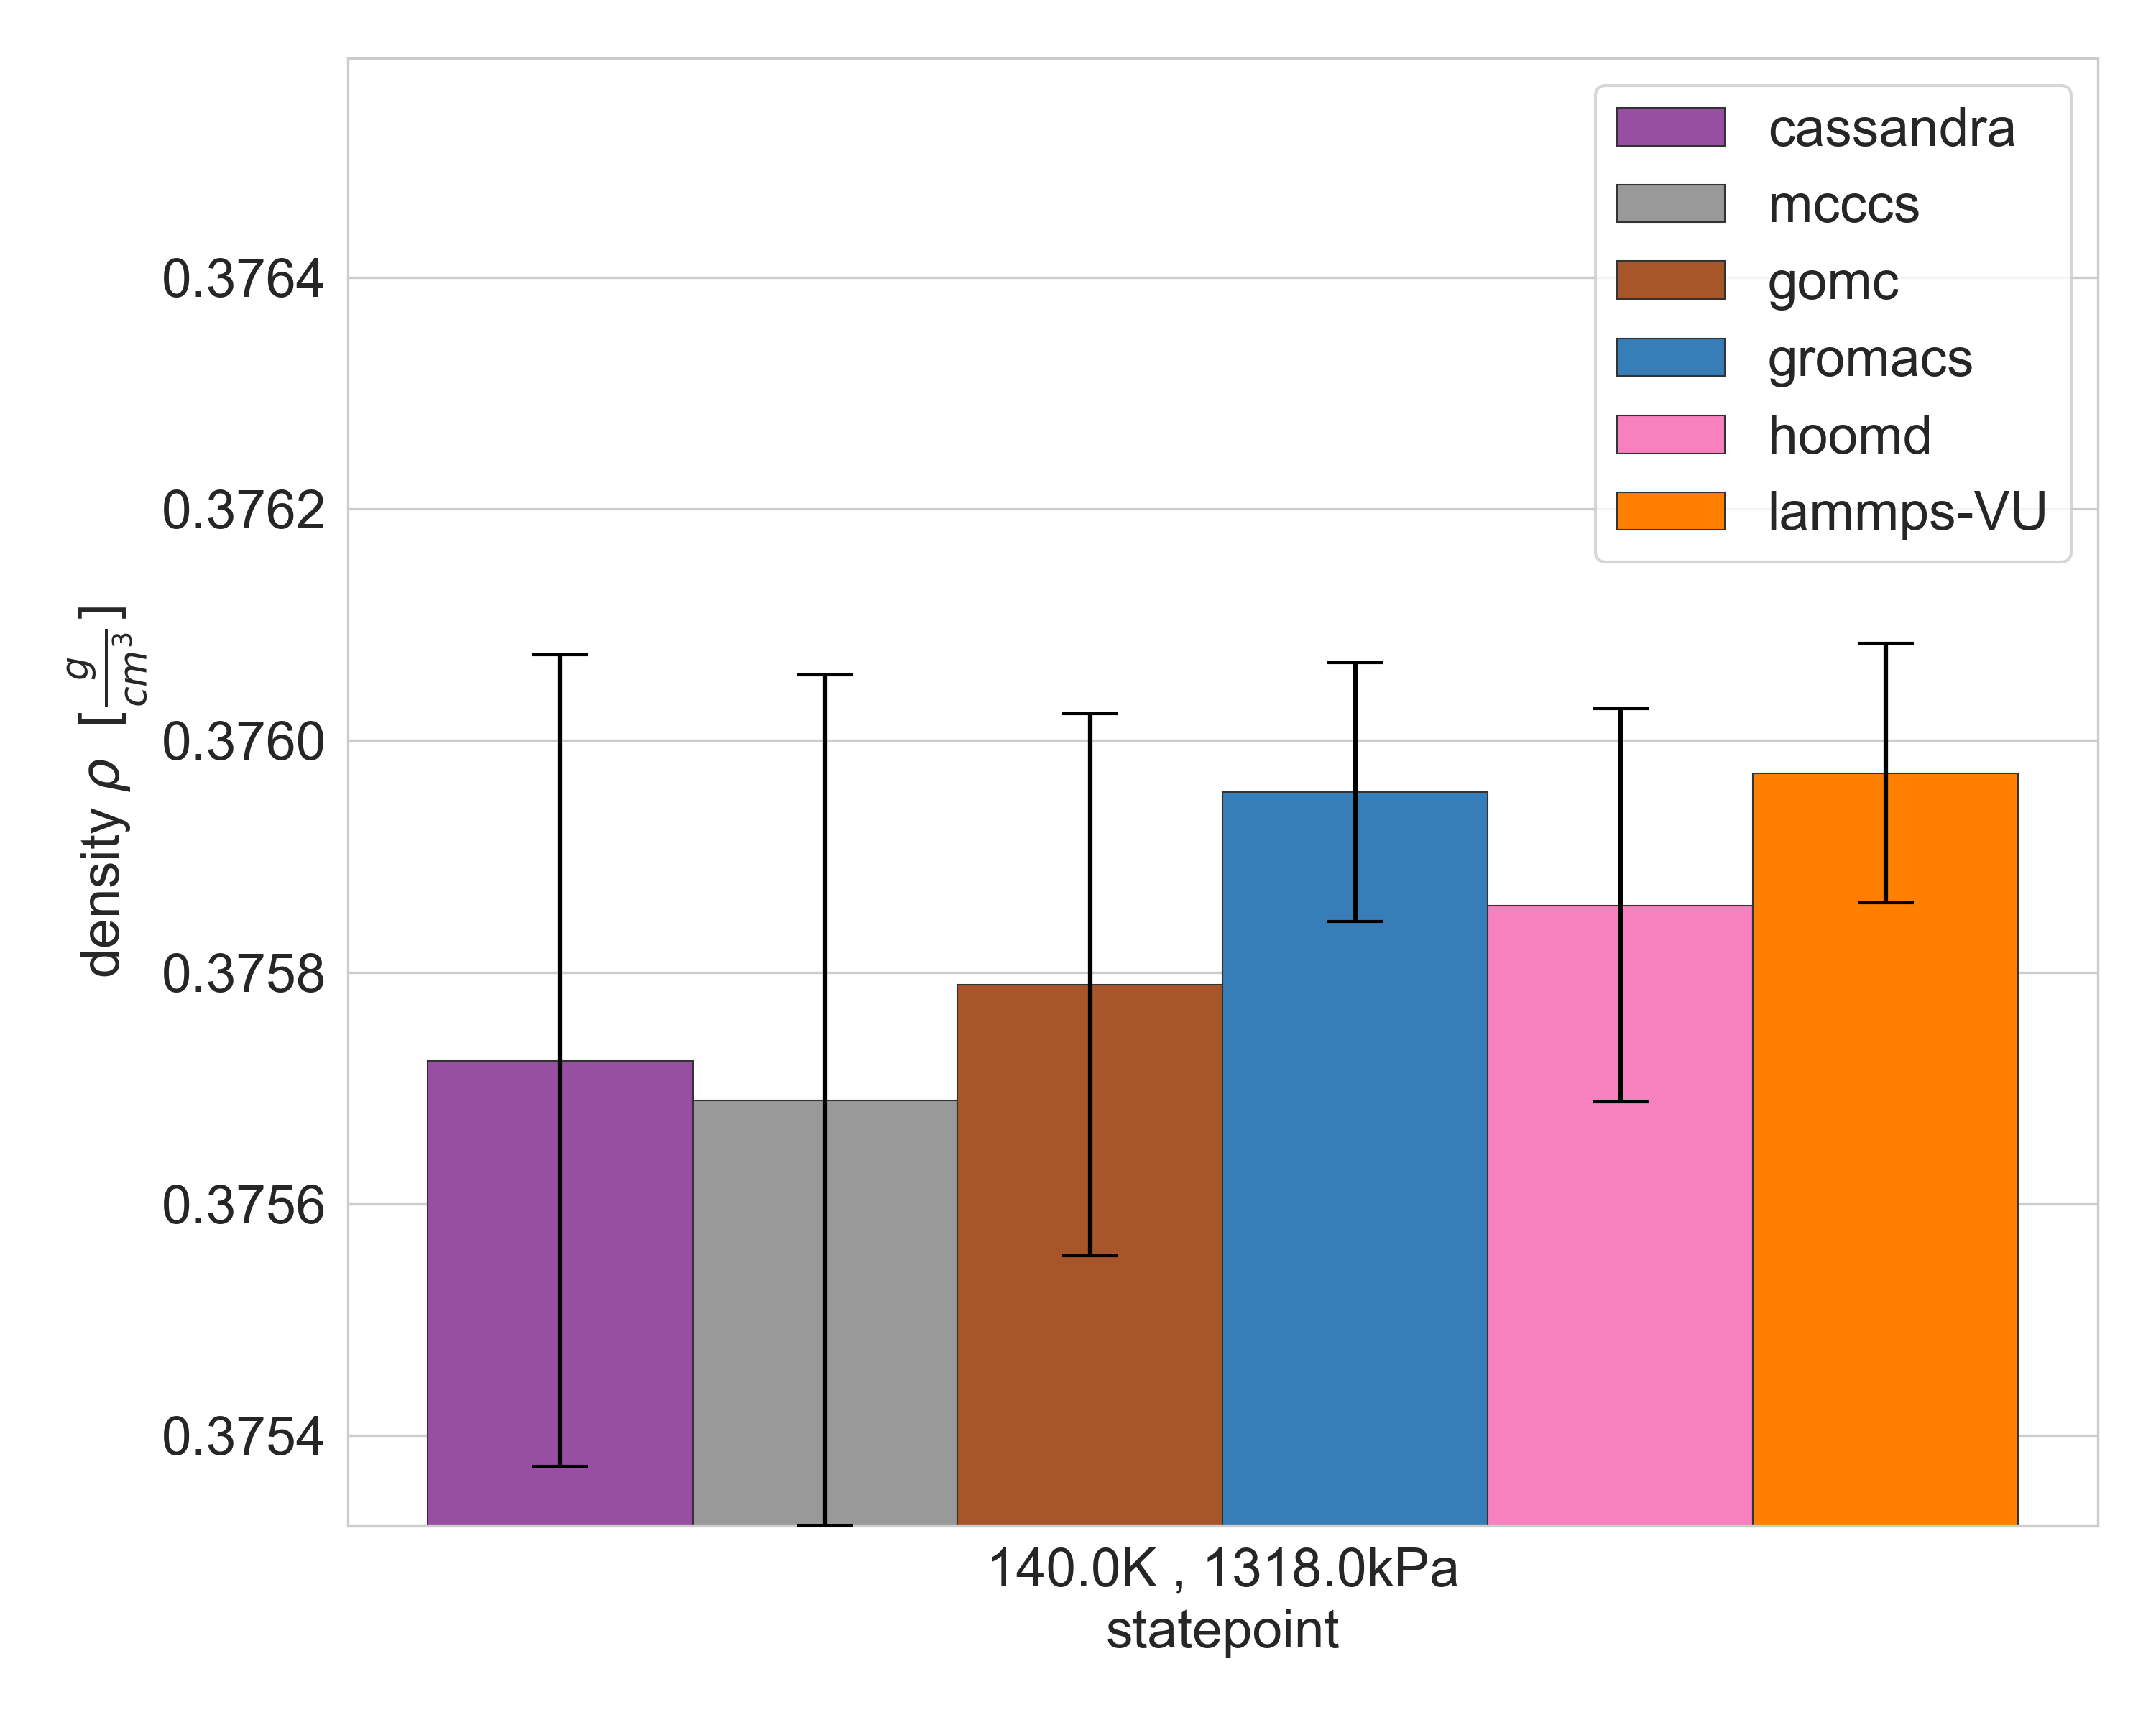
\includegraphics[width=0.8\linewidth,keepaspectratio]{figures/rep_study/methaneUA_summary.png}
    \caption{Average density of methane by engine. Average of independent samples from equilibrated regions of 16 replicates. Error bars represent two standard deviations.}\label{fig:methane_density}
\end{figure}

\begin{figure}[h!]
    \centering
    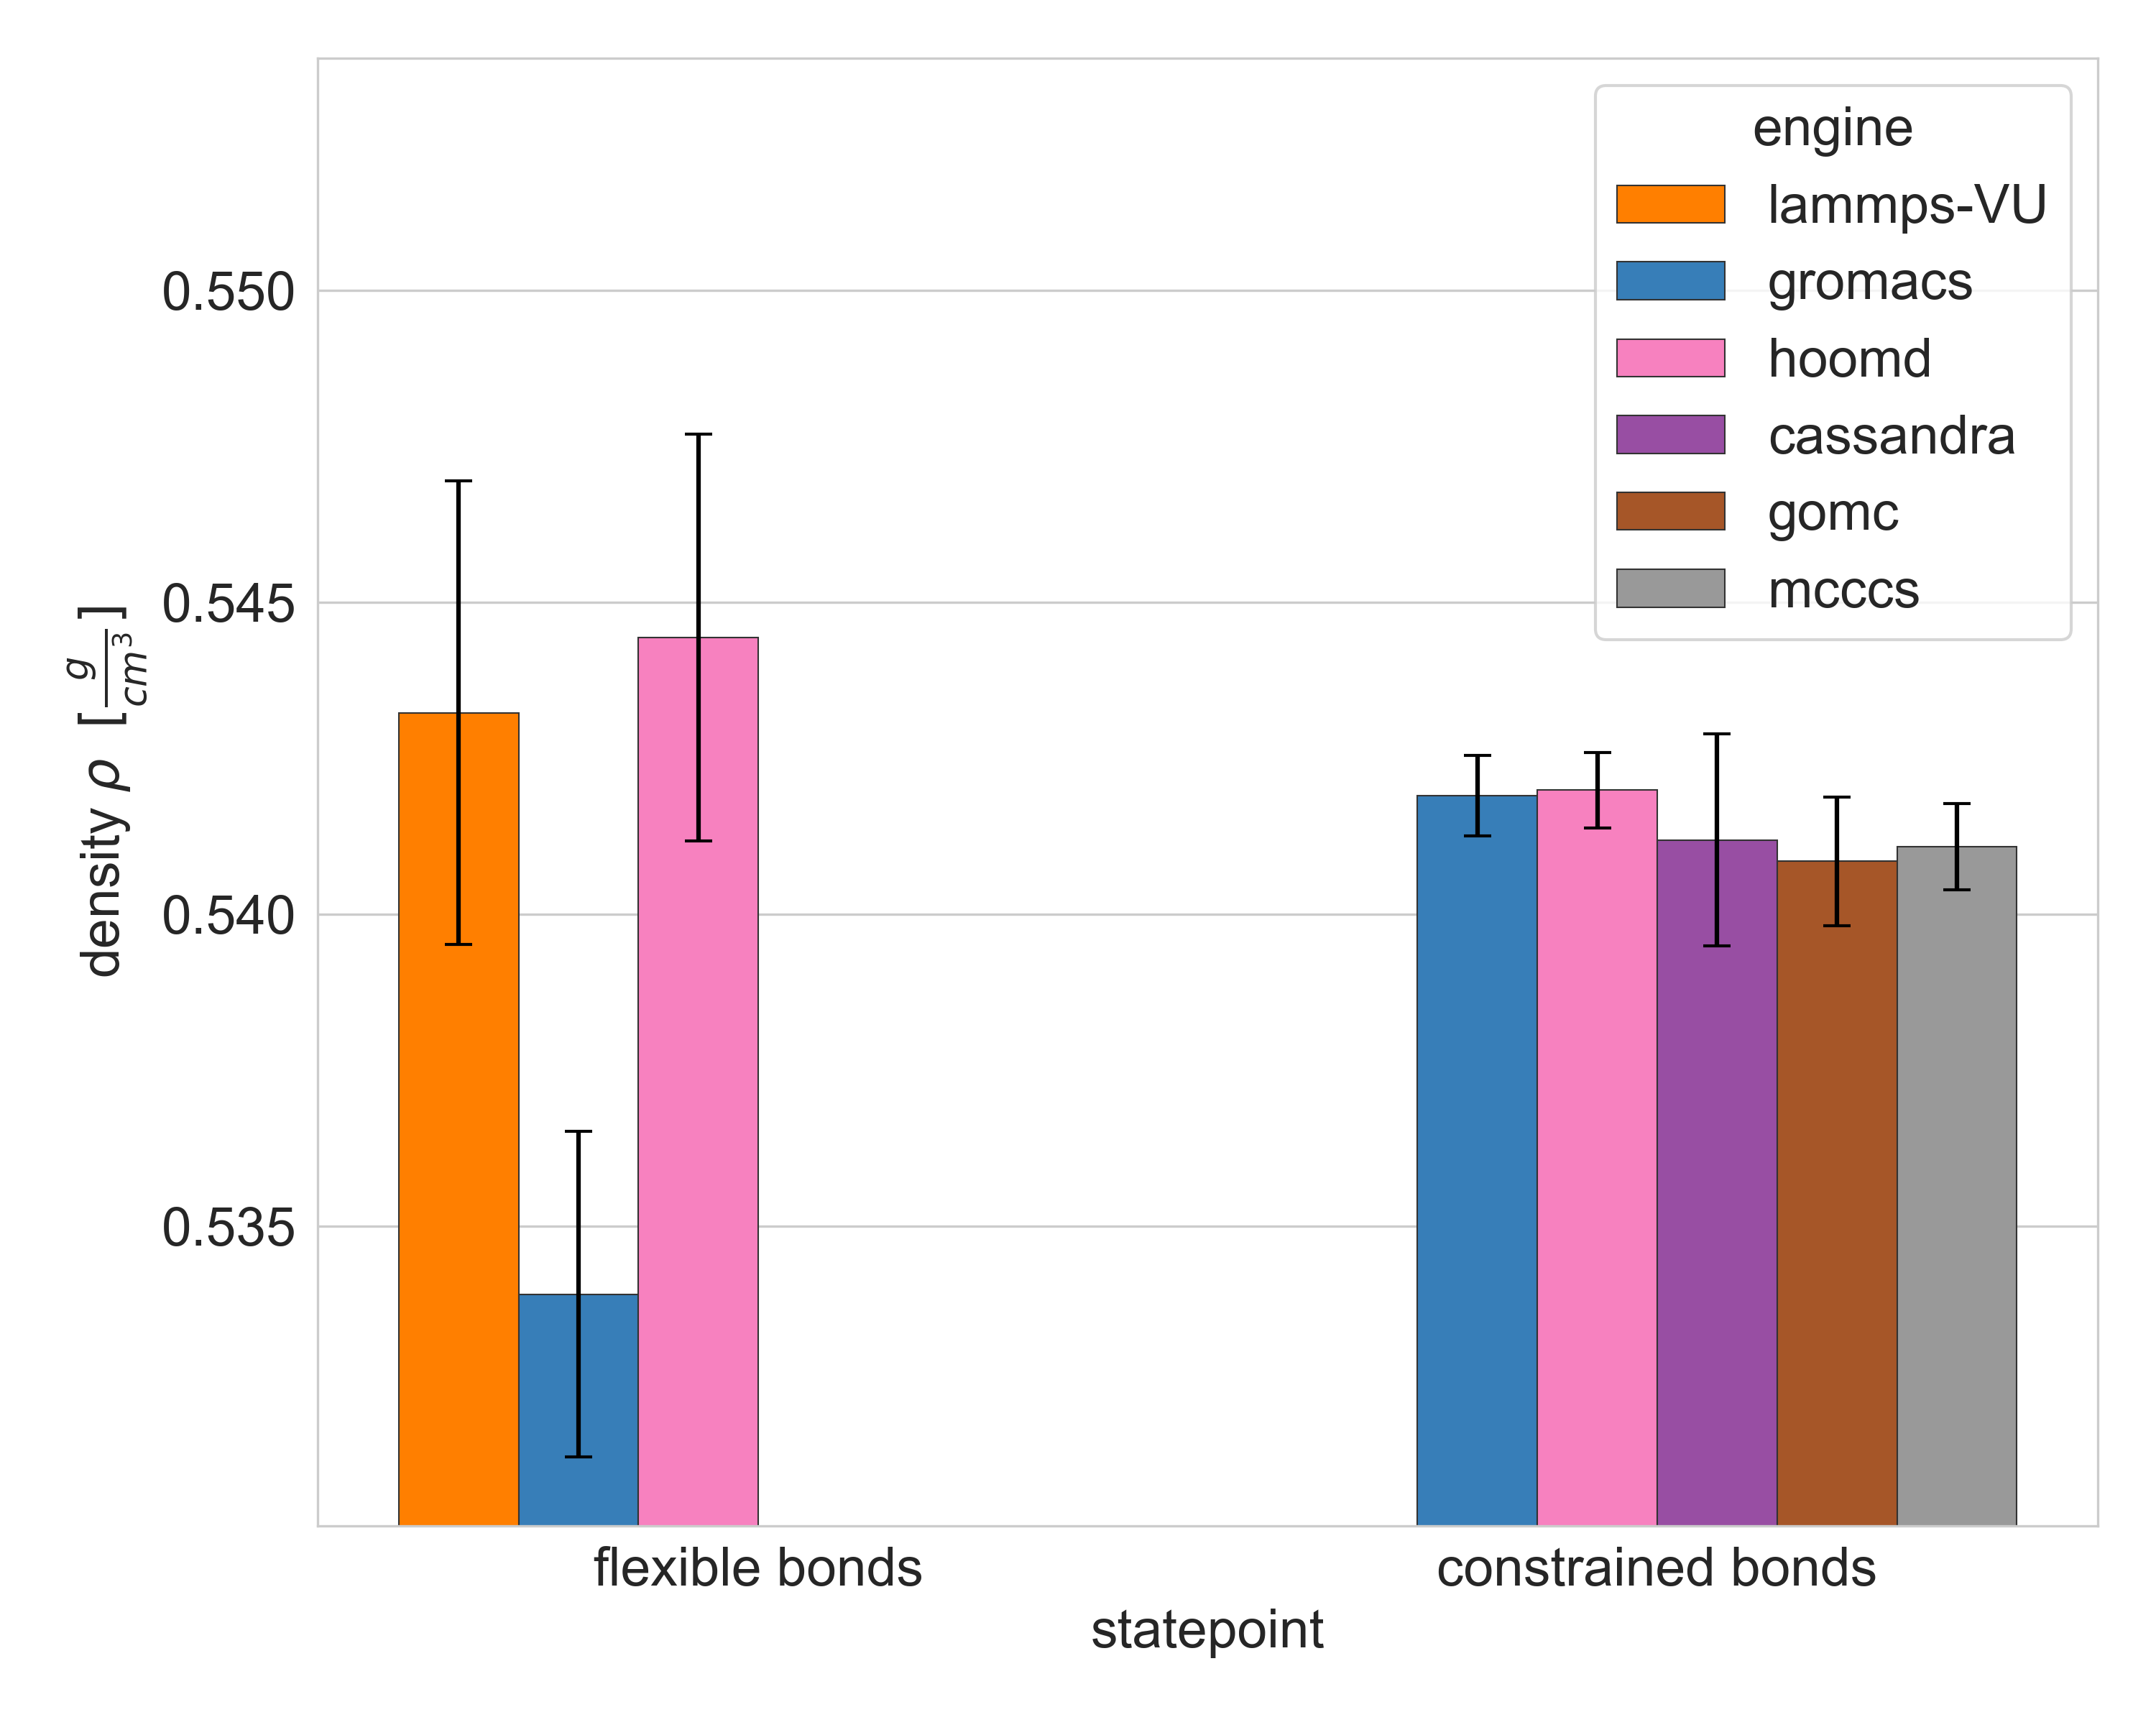
\includegraphics[width=0.8\linewidth,keepaspectratio]{figures/rep_study/pentane_summary.png}
    \caption{Average density of pentane with flexible or constrained bonds by engine. Average of independent samples from equilibrated regions of 16 replicates. Error bars represent two standard deviations.}\label{fig:pentane_constrain_density}
\end{figure}

\begin{figure}[h!]
    \centering
    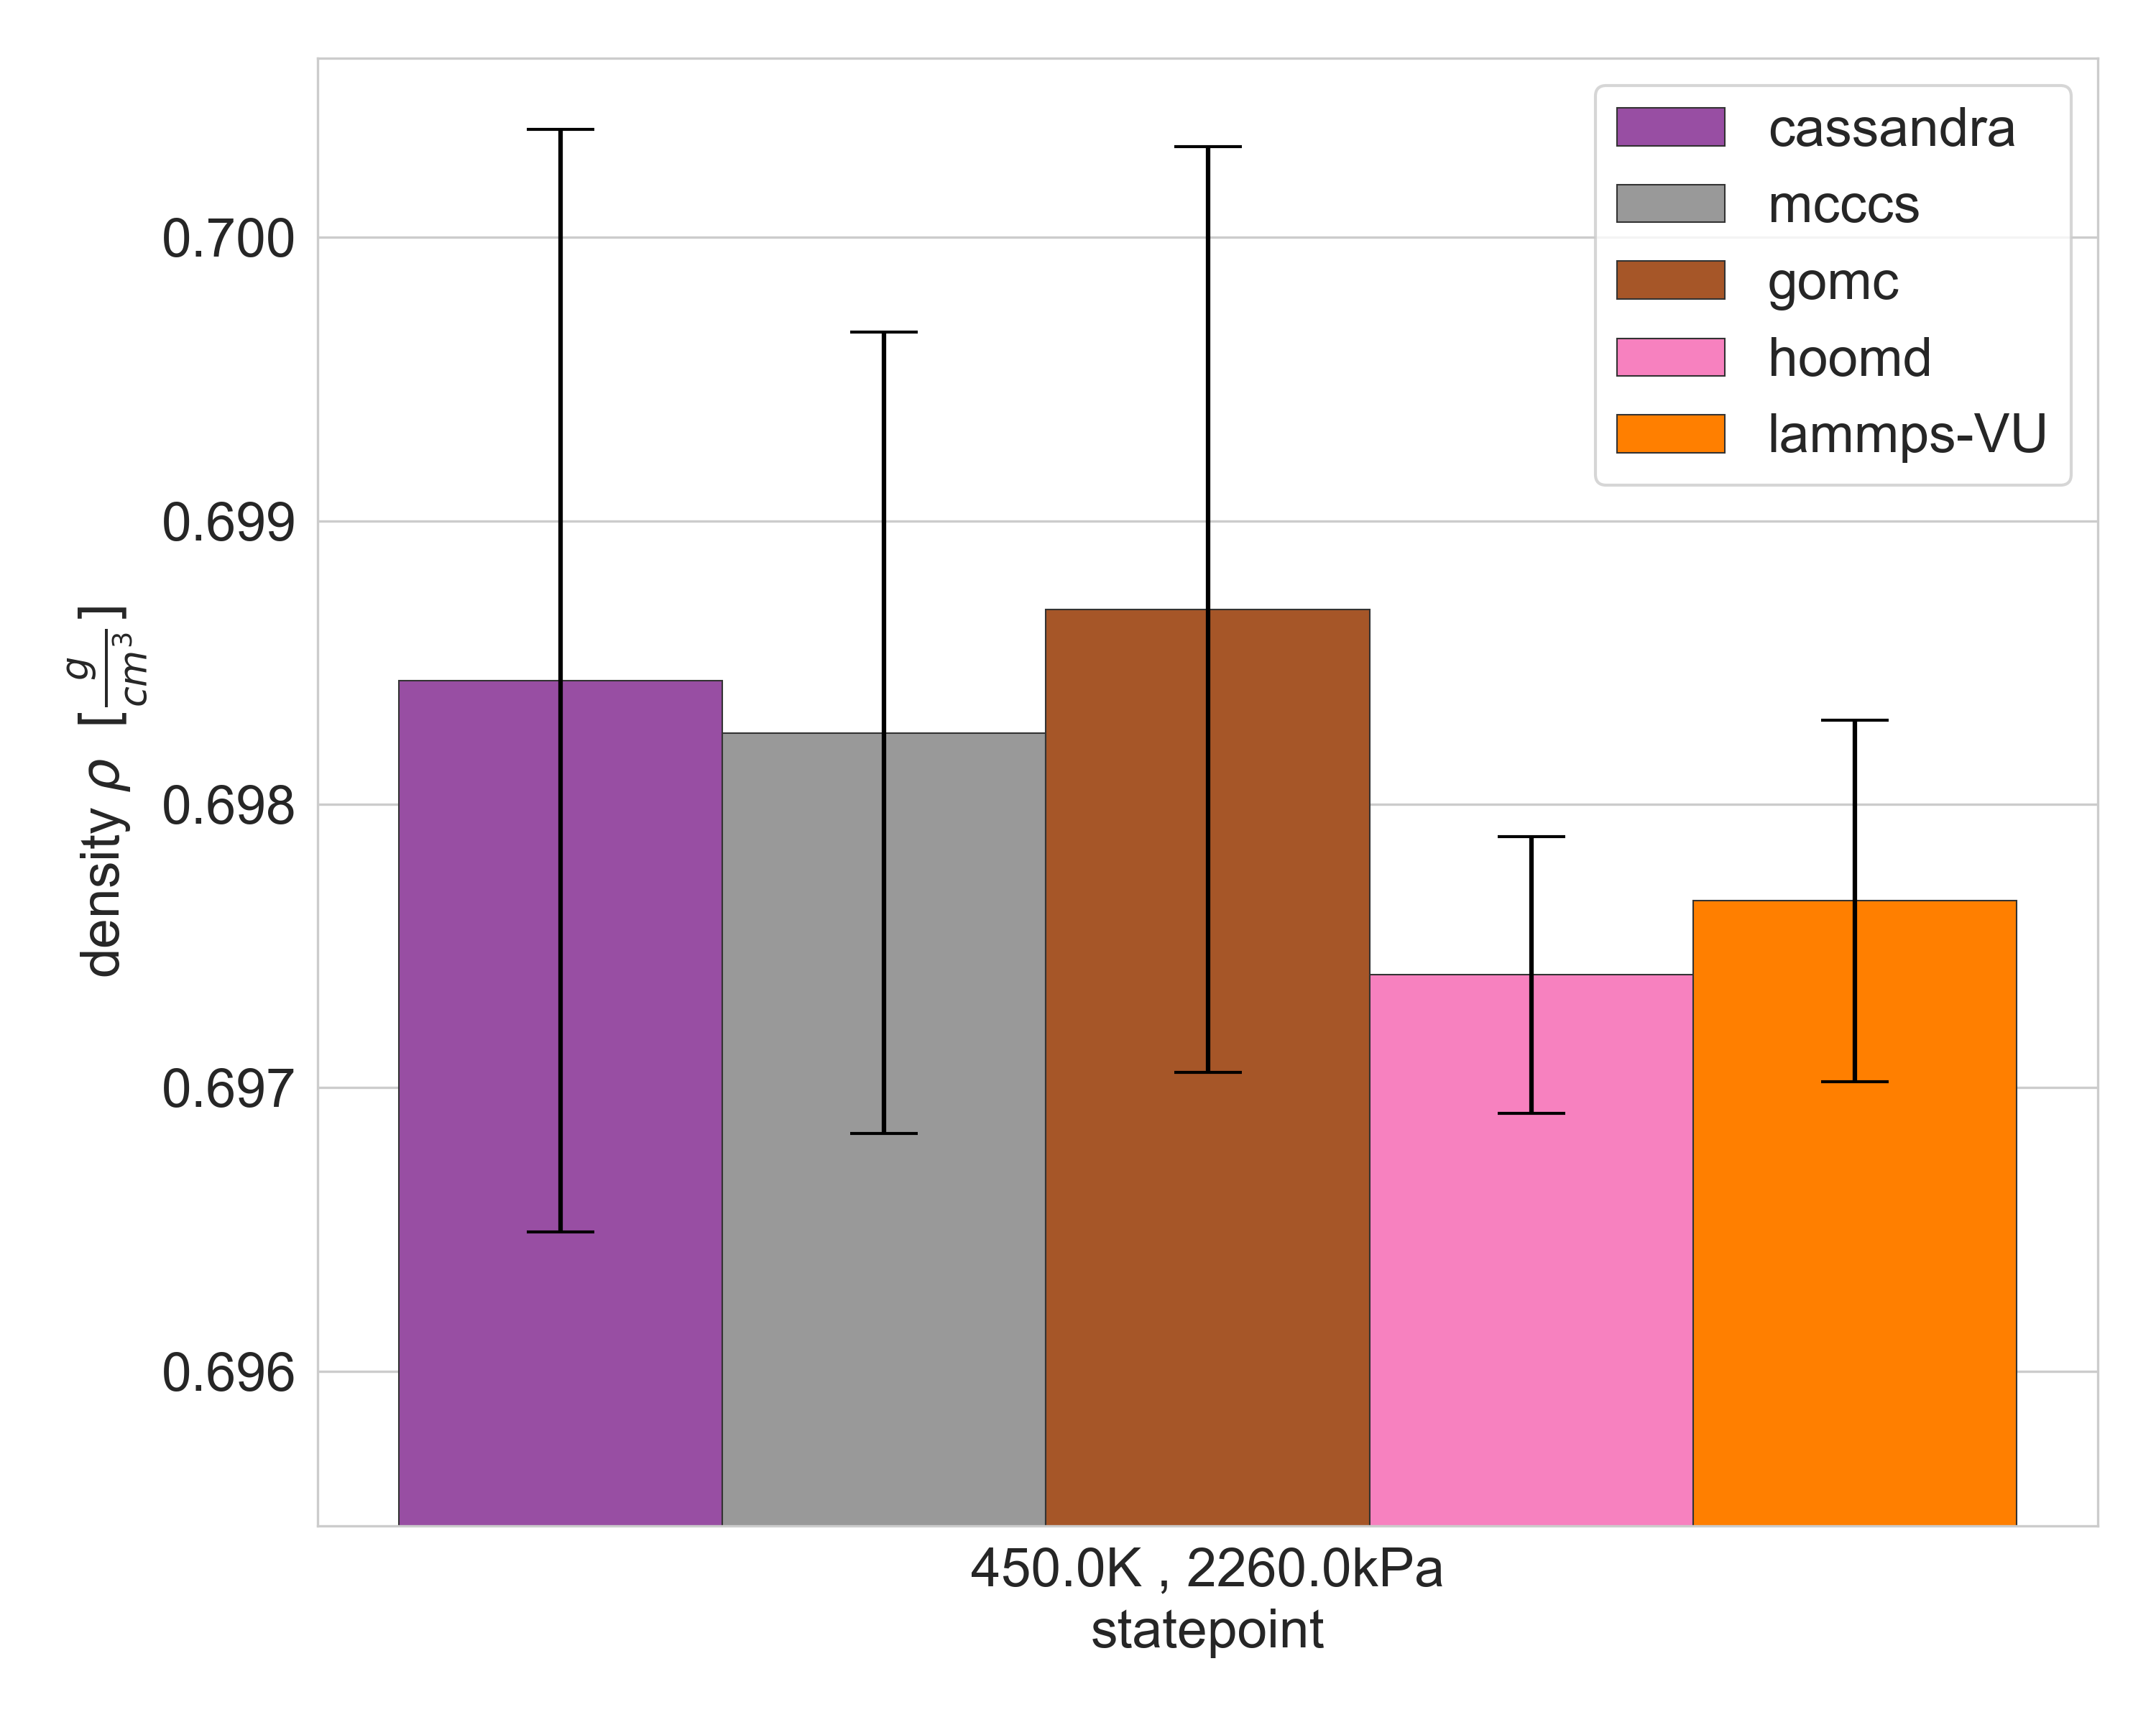
\includegraphics[width=0.8\linewidth,keepaspectratio]{figures/rep_study/benzeneUA_summary.png}
    \caption{Average density of benzene by engine. Average of independent samples from equilibrated regions of 16 replicates. Error bars represent two standard deviations.}\label{fig:benzene_density}
\end{figure}

\begin{figure}[h!]
    \centering
    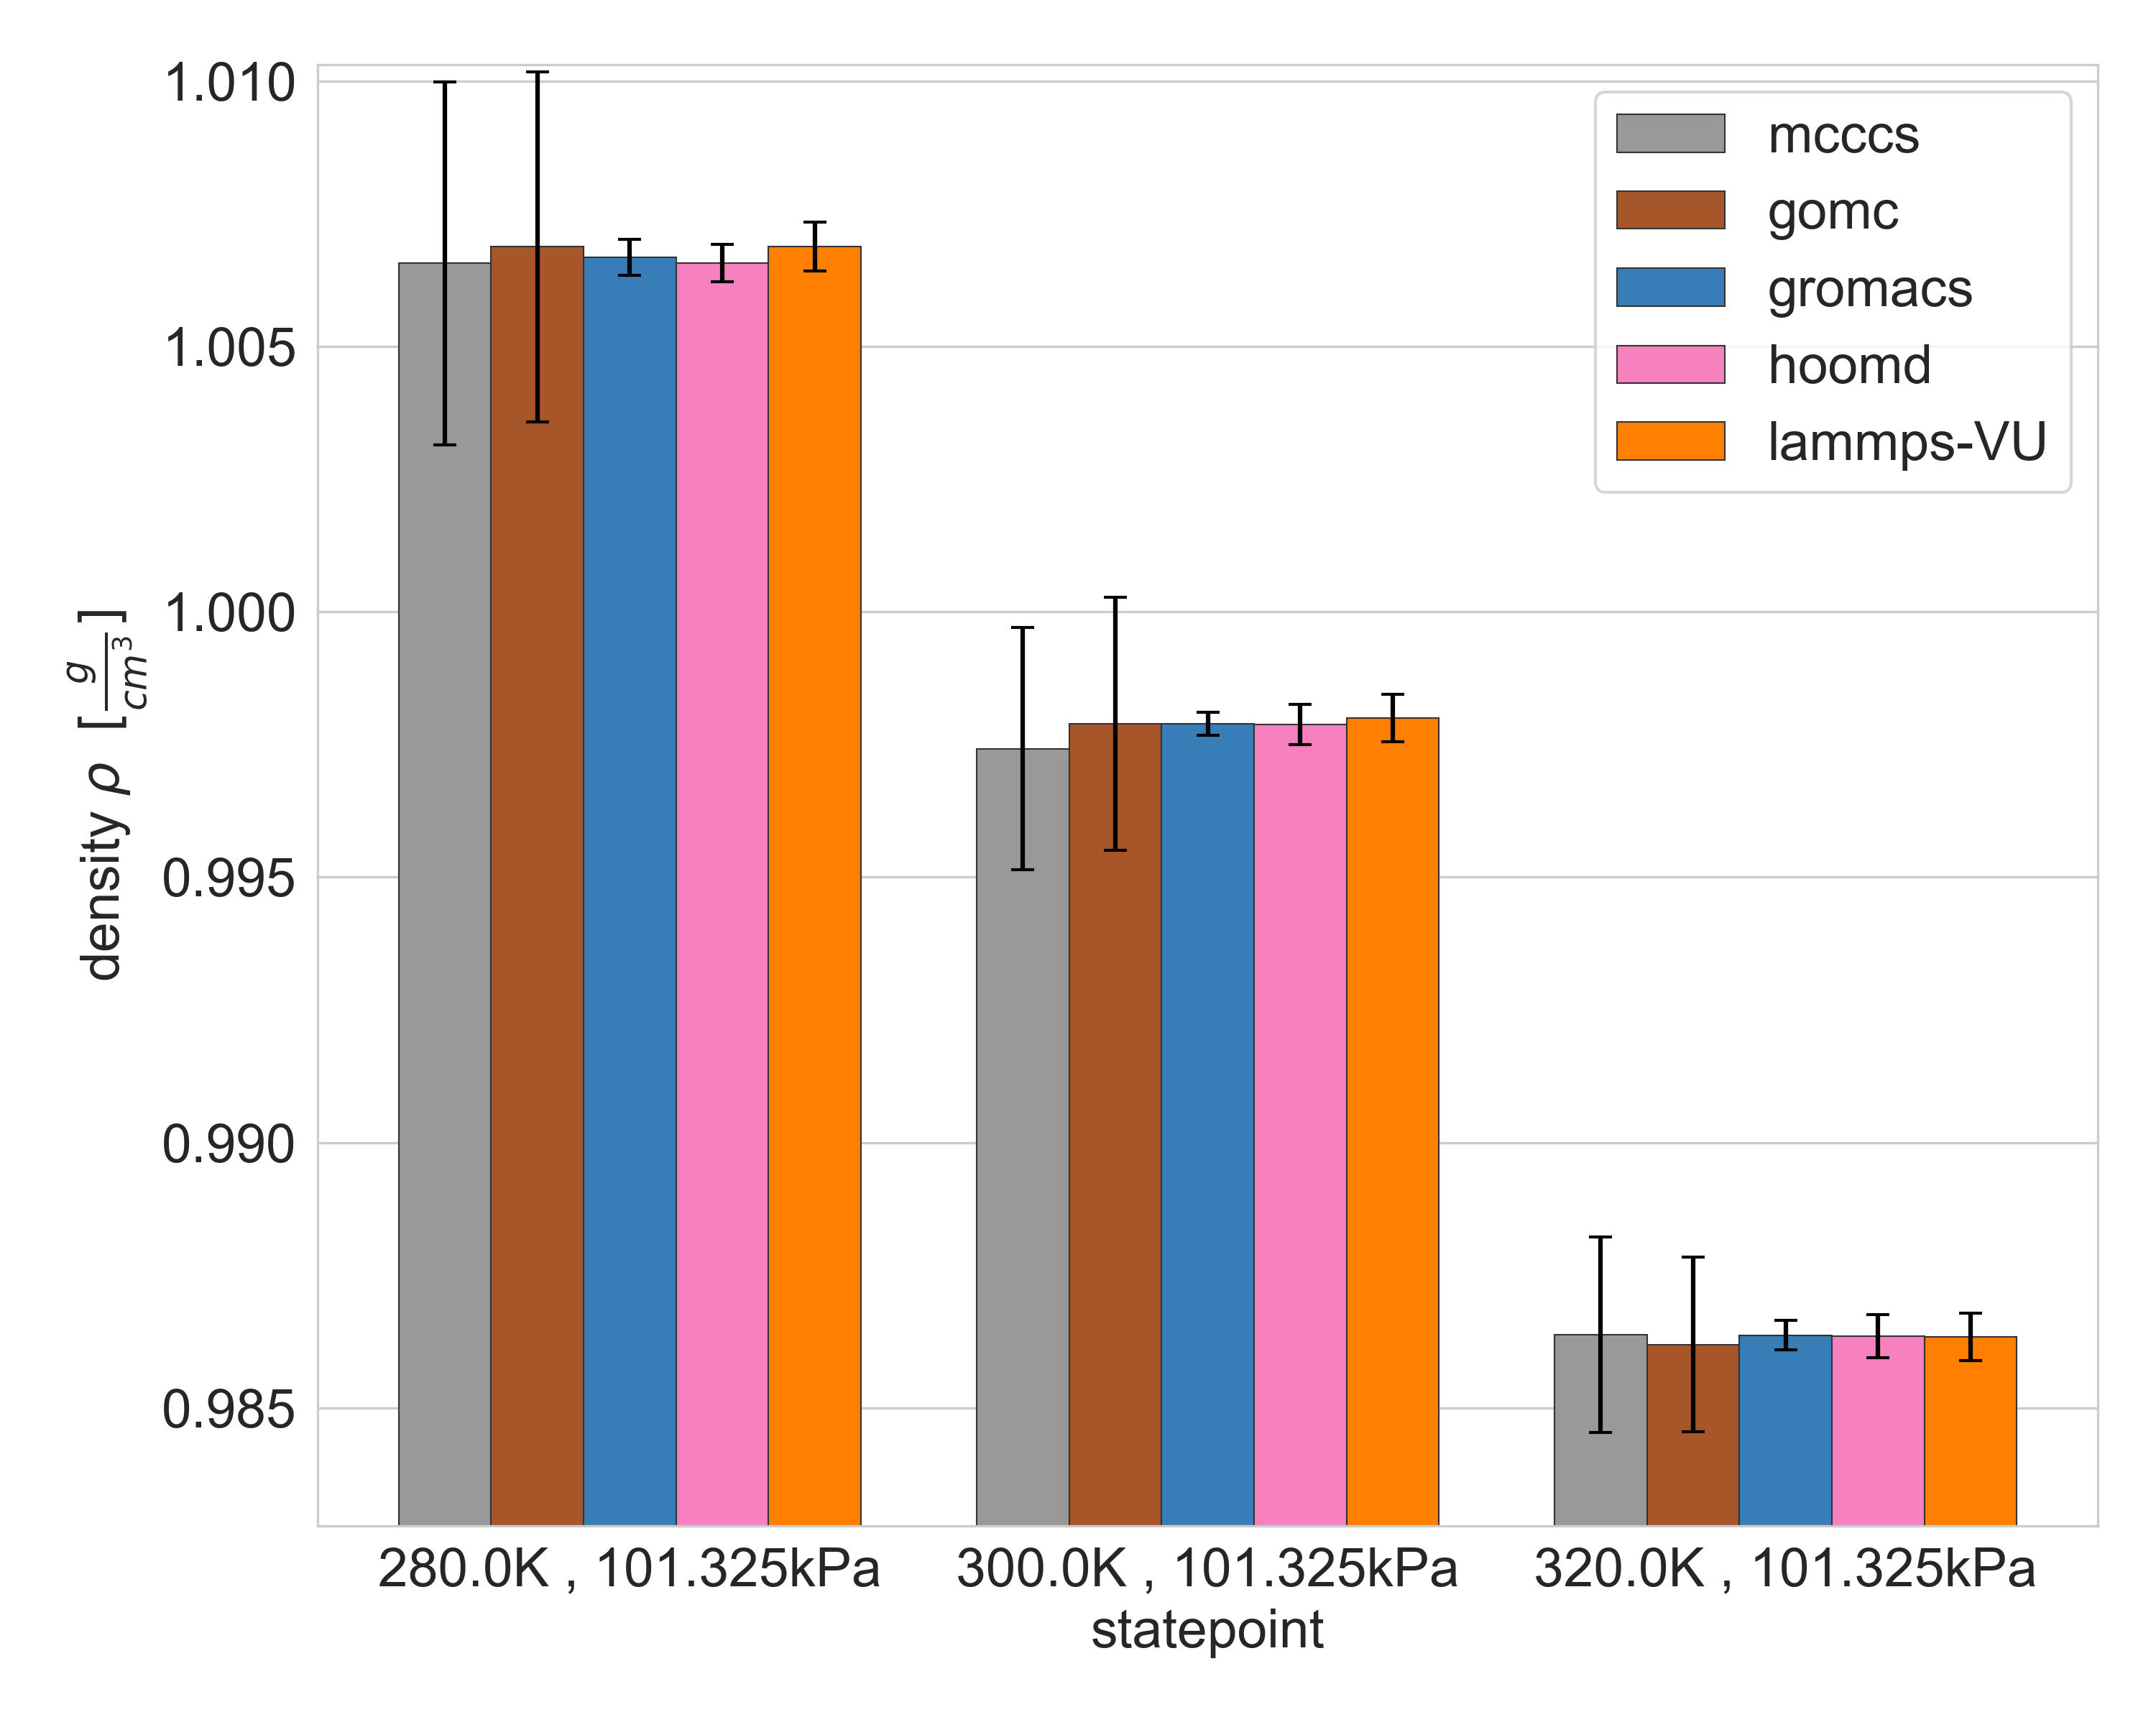
\includegraphics[width=0.8\linewidth,keepaspectratio]{figures/rep_study/waterSPCE_summary.png}
    \caption{Average density of water at three statepoints by engine. Average of independent samples from equilibrated regions of 16 replicates. Error bars represent two standard deviations.}\label{fig:water_density}
\end{figure}

\begin{figure}[h!]
    \centering
    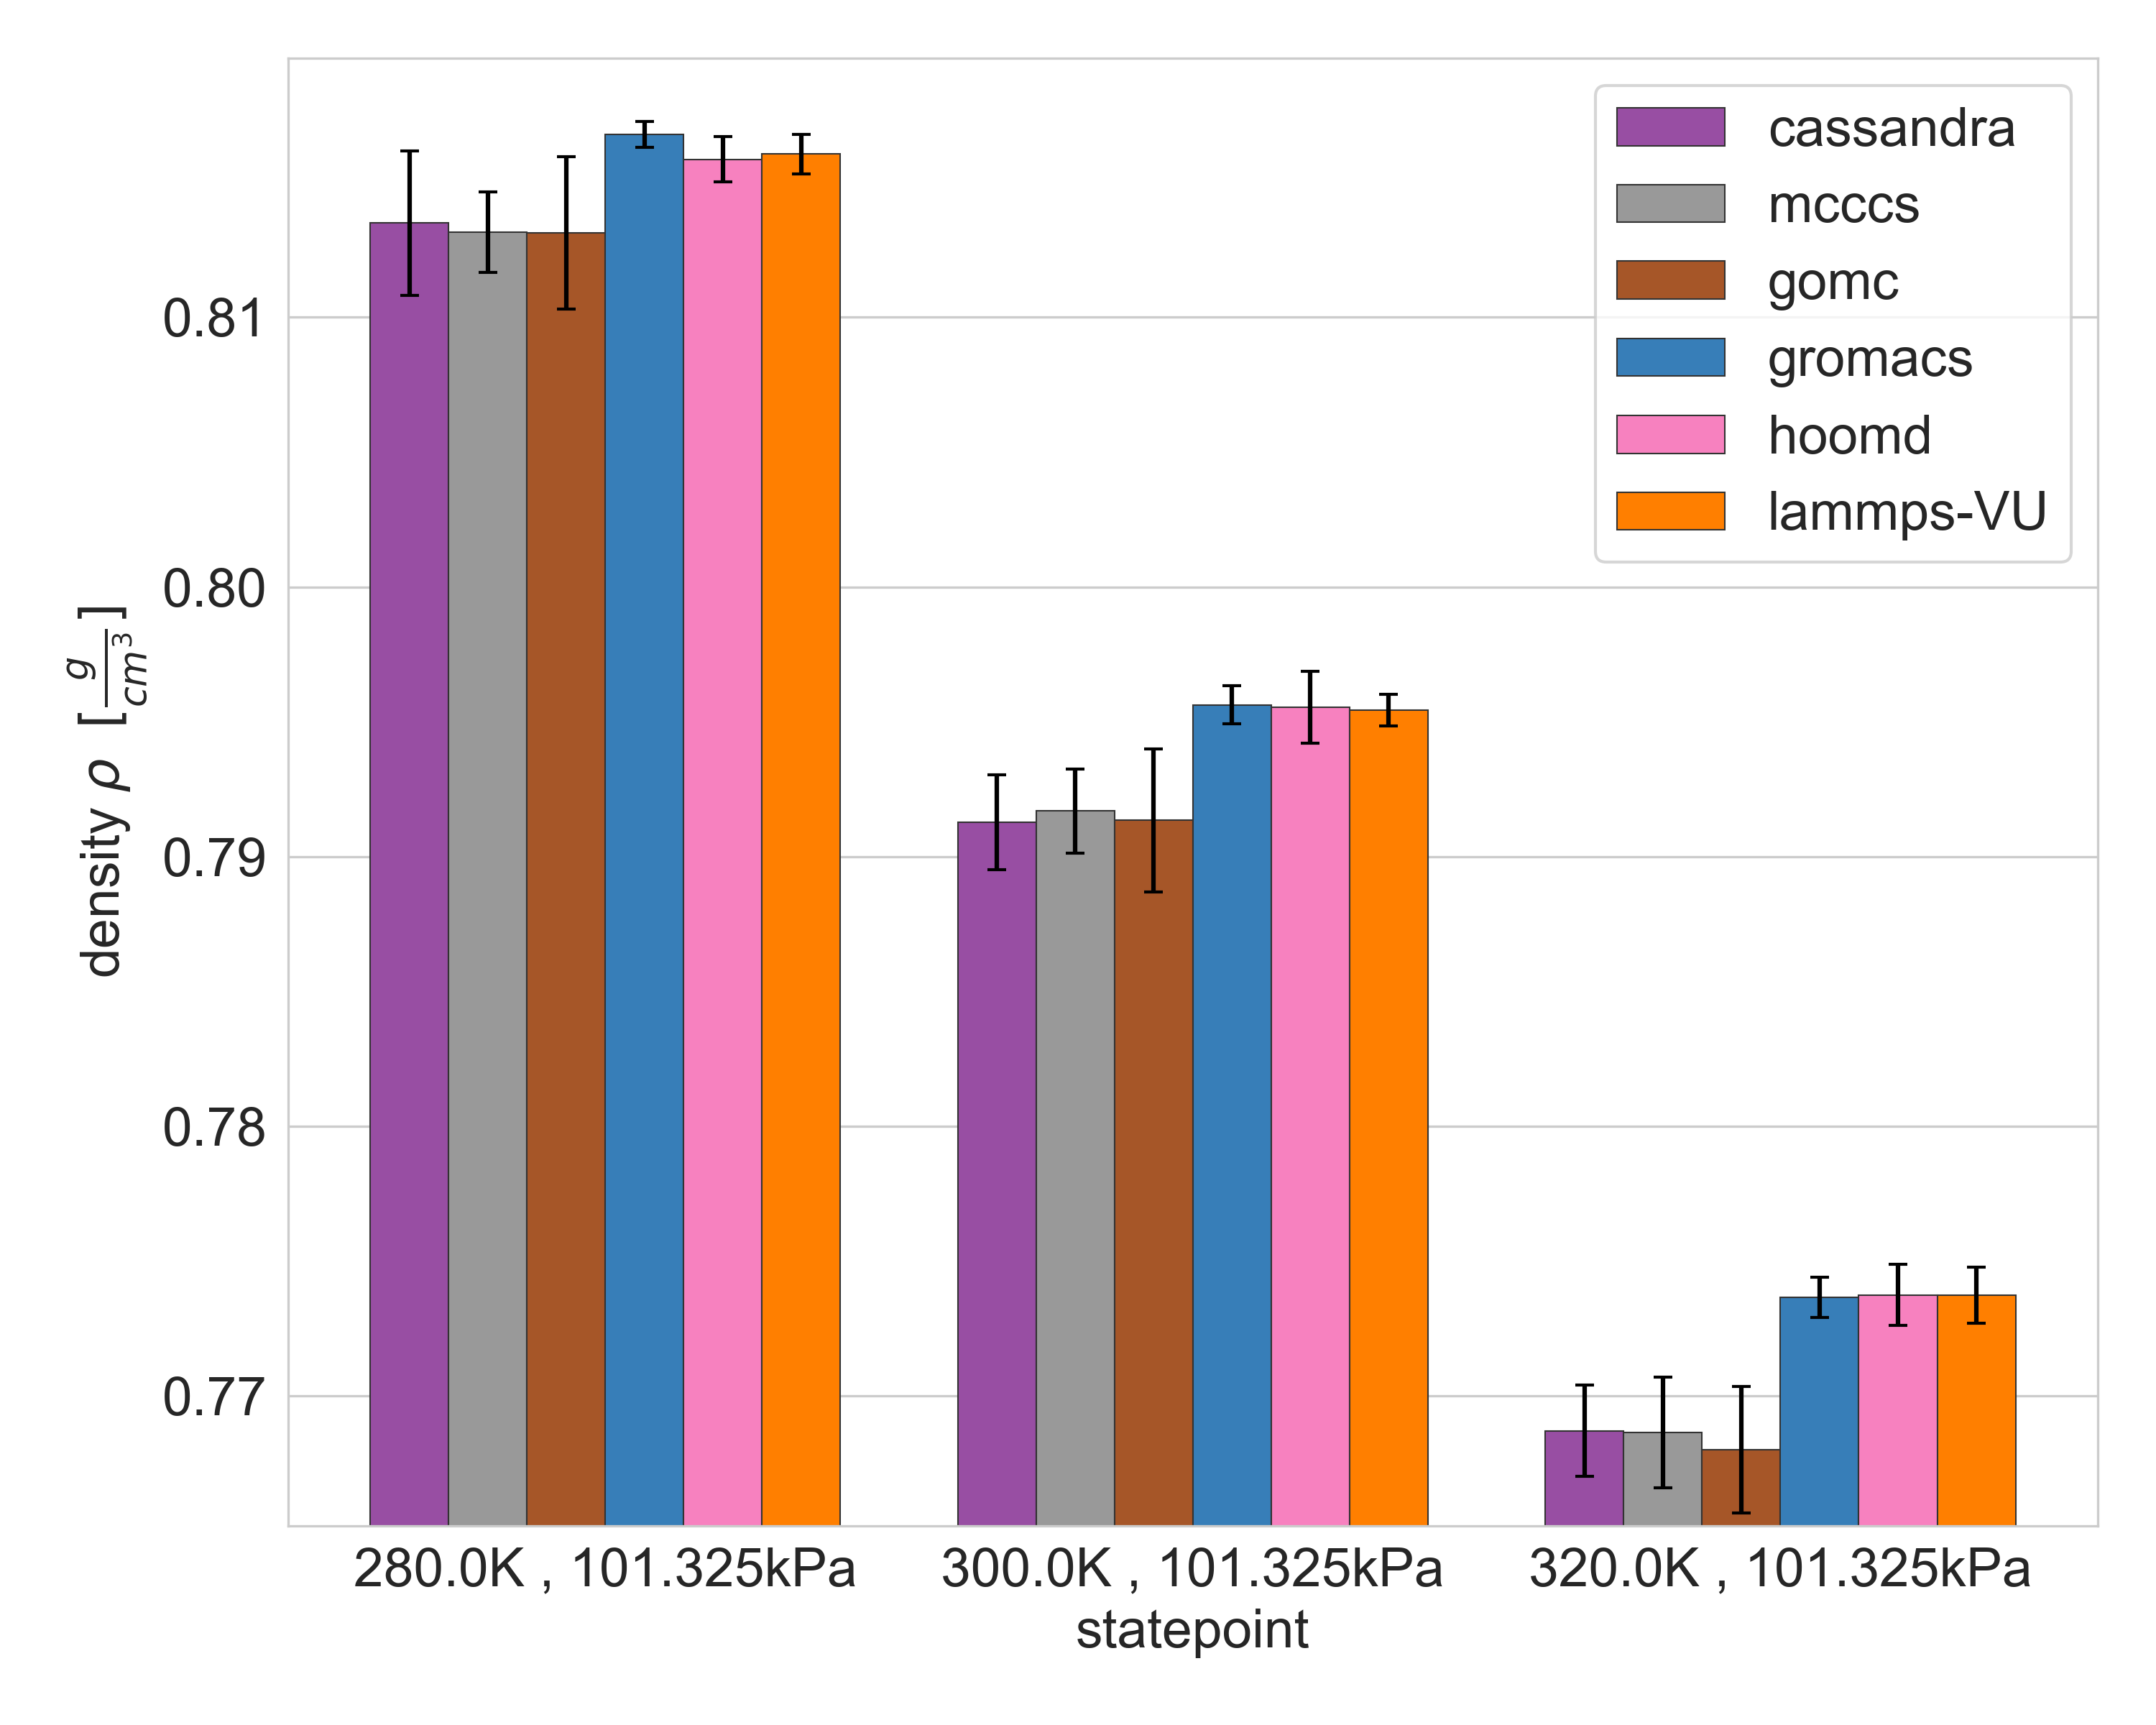
\includegraphics[width=0.8\linewidth,keepaspectratio]{figures/rep_study/ethanolAA_summary.png}
    \caption{Average density of ethanol by engine. Average of independent samples from equilibrated regions of 16 replicates. Error bars represent two standard deviations.}\label{fig:ethanol_density}
\end{figure}

MC in general has lower density and greater variability.

Most results agree within error.

pentane flexible vs constrained: MC engines can only run constrained bonds. within the same engine and same system (pentane) have higher density than with the constrained bonds. This may explain the lower density found in MC.


\section{Conclusions}
Beyond just an opportunity to validate that our results were "right," working on this project together with other simulators with different backgrounds and expertise was an invaluable opportunity to learn.

